%%
%% This is file `sample-authordraft.tex',
%% generated with the docstrip utility.
%%
%% The original source files were:
%%
%% samples.dtx  (with options: `authordraft')
%% 
%% IMPORTANT NOTICE:
%% 
%% For the copyright see the source file.
%% 
%% Any modified versions of this file must be renamed
%% with new filenames distinct from sample-authordraft.tex.
%% 
%% For distribution of the original source see the terms
%% for copying and modification in the file samples.dtx.
%% 
%% This generated file may be distributed as long as the
%% original source files, as listed above, are part of the
%% same distribution. (The sources need not necessarily be
%% in the same archive or directory.)
%%
%% The first command in your LaTeX source must be the \documentclass command.
\documentclass[sigconf]{acmart}
% NOTE that a single column version is required for submission and peer review. This can be done by changing the \doucmentclass[...]{acmart} in this template to 
% \documentclass[manuscript,screen]{acmart}

%%
%% \BibTeX command to typeset BibTeX logo in the docs
\AtBeginDocument{%
  \providecommand\BibTeX{{%
    \normalfont B\kern-0.5em{\scshape i\kern-0.25em b}\kern-0.8em\TeX}}}

%% Rights management information.  This information is sent to you
%% when you complete the rights form.  These commands have SAMPLE
%% values in them; it is your responsibility as an author to replace
%% the commands and values with those provided to you when you
%% complete the rights form.
\copyrightyear{2020}
\acmYear{2020}
\setcopyright{acmlicensed}
\acmConference[COMPASS '20]{ACM SIGCAS Conference on Computing and Sustainable Societies (COMPASS)}{June 15--17, 2020}{Ecuador}
\acmBooktitle{ACM SIGCAS Conference on Computing and Sustainable Societies (COMPASS) (COMPASS '20), June 15--17, 2020, Ecuador}
\acmPrice{15.00}
\acmDOI{10.1145/3378393.3402285}
\acmISBN{978-1-4503-7129-2/20/06}

%%
%% Submission ID.
%% Use this when submitting an article to a sponsored event. You'll
%% receive a unique submission ID from the organizers
%% of the event, and this ID should be used as the parameter to this command.
%%\acmSubmissionID{123-A56-BU3}
% Load basic packages
\usepackage{balance}       % to better equalize the last page
\usepackage{graphics}      % for EPS, load graphicx instead 
\usepackage[T1]{fontenc}   % for umlauts and other diaeresis
\usepackage{txfonts}
\usepackage{mathptmx}
\usepackage{booktabs}
\usepackage{textcomp}
\usepackage{array}
\usepackage{caption}
\usepackage{color}
% Some optional stuff you might like/need.
\usepackage{microtype}        % Improved Tracking and Kerning
% \usepackage[all]{hypcap}    % Fixes bug in hyperref caption linking
\usepackage{ccicons}          % Cite your images correctly!
% \usepackage[utf8]{inputenc} % for a UTF8 editor only
%%
%% The majority of ACM publications use numbered citations and
%% references.  The command \citestyle{authoryear} switches to the
%% "author year" style.
%%
%% If you are preparing content for an event
%% sponsored by ACM SIGGRAPH, you must use the "author year" style of
%% citations and references.
%% Uncommenting
%% the next command will enable that style.
%%\citestyle{acmauthoryear}

%%
%% end of the preamble, start of the body of the document source.
\begin{document}

%%
%% The "title" command has an optional parameter,
%% allowing the author to define a "short title" to be used in page headers.
\title{LokDhaba : Acquiring, Visualizing and Disseminating Data on Indian Elections}


%%
%% The "author" command and its associated commands are used to define
%% the authors and their affiliations.
%% Of note is the shared affiliation of the first two authors, and the
%% "authornote" and "authornotemark" commands
%% used to denote shared contribution to the research.
\author{Mohit Kumar}
\email{mohit.kumar@ashoka.edu.in}
\affiliation{%
  \institution{Trivedi Centre for Political Data, Ashoka University}
  \state{Haryana}
  \country{India}
}

\author{Chinmay Narayan}
\email{chinmay.narayan@amuselabs.com}
\affiliation{%
  \institution{Amuse Labs} 
  \city{Uttarakhand}
  \country{India}
}

\author{Sudheendra Hangal}
\email{sudheendra.hangal@ashoka.edu.in}
\affiliation{%
  \institution{Trivedi Centre for Political Data, Ashoka University}
  \state{Haryana}
  \country{India}
}

\author{Priyamvada Trivedi}
\email{priyamvada.trivedi@ashoka.edu.in}
\affiliation{%
 \institution{Trivedi Centre for Political Data, Ashoka University}
  \state{Haryana}
  \country{India}
}

%%
%% By default, the full list of authors will be used in the page
%% headers. Often, this list is too long, and will overlap
%% other information printed in the page headers. This command allows
%% the author to define a more concise list
%% of authors' names for this purpose.
\renewcommand{\shortauthors}{Kumar and Narayan, et al.}

%%
%% The abstract is a short summary of the work to be presented in the
%% article.
\begin{abstract}
  Despite the importance of elections in India, the world's largest democracy, data on Indian electoral outcomes has not been easily available for political analysis in the past. This has been due to the problems inherent in assembling any data archive of social and political data spanning many decades. In this paper, we shed some light on these problems and present some solutions in the context of a system we built called LokDhaba. LokDhaba includes the first freely-available, structured and cleaned data archive on Indian electoral outcomes at the national or state level from 1962 onwards. To build this archive, we overcame the challenges of data scraping, parsing, cleaning, consistency checking and integration between multiple sources, with the help of some novel tools. LokDhaba is being used extensively by political scientists, researchers, journalists and others to better understand long-term electoral trends in India.
\end{abstract}

%%
%% The code below is generated by the tool at http://dl.acm.org/ccs.cfm.
%% Please copy and paste the code instead of the example below.
%%
\begin{CCSXML}
<ccs2012>
   <concept>
       <concept_id>10002951.10003317.10003318</concept_id>
       <concept_desc>Information systems~Document representation</concept_desc>
       <concept_significance>300</concept_significance>
       </concept>
   <concept>
       <concept_id>10002951.10002952.10002953.10002955</concept_id>
       <concept_desc>Information systems~Relational database model</concept_desc>
       <concept_significance>300</concept_significance>
       </concept>
   <concept>
       <concept_id>10002951.10003227.10003233</concept_id>
       <concept_desc>Information systems~Collaborative and social computing systems and tools</concept_desc>
       <concept_significance>500</concept_significance>
       </concept>
   <concept>
       <concept_id>10010147.10010178.10010187</concept_id>
       <concept_desc>Computing methodologies~Knowledge representation and reasoning</concept_desc>
       <concept_significance>500</concept_significance>
       </concept>
 </ccs2012>
\end{CCSXML}

\ccsdesc[300]{Information systems~Document representation}
\ccsdesc[300]{Information systems~Relational database model}
\ccsdesc[500]{Information systems~Collaborative and social computing systems and tools}
\ccsdesc[500]{Computing methodologies~Knowledge representation and reasoning}

%%
%% Keywords. The author(s) should pick words that accurately describe
%% the work being presented. Separate the keywords with commas.
\keywords{social database design; data visualization; web application.}

%% A "teaser" image appears between the author and affiliation
%% information and the body of the document, and typically spans the
%% page.

%%
%% This command processes the author and affiliation and title
%% information and builds the first part of the formatted document.
\maketitle


\section{Introduction}

The Indian elections are the largest in the world, currently involving an electorate of over 900 million people~\cite{quraishi2014undocumented}.  As specified in the Indian constitution, elections are held every five years at national (parliamentary), state and local levels, with a ``First Past The Post'' system. At the state and parliamentary level, the elections are conducted by the Election Commission of India (ECI) and the state election commissions in 29 states and 7 union territories. These elections generate a fascinating trove of data for understanding political trends and processes. However, it is difficult to obtain structured data for the outcomes of Indian elections in consistent formats over a long period of time. This inhibits fundamental questions political scientists would like to ask, such as: What is the pattern in voter turnout over time across the country? Are women participating more, or less, in the political process? Is the supply of political candidates increasing or decreasing over time? How many times does an aspirant for political office contest an election? Are these patterns correlated with caste, geography, age, gender or income?

In this paper, we discuss technical challenges we encountered in the acquisition and dissemination of Indian elections data that enables the answer to such questions. Over the past three years, we have set up a unique data processing pipeline to process the results of all Indian elections since 1962 and make them freely available to researchers, journalists and the general public. Our dataset includes cleaned and harmonized electoral results published by the ECI, new primary variables (such as unique identifiers for all individuals contesting Indian elections), and integration with datasets from other reliable sources such as the Association of Democratic Reforms (ADR), PRS Legislative Research and the Lok Sabha (the lower house of the Indian Parliament). Over this period, we have managed to keep our dataset up to date, and absorbed the results of over 20 state elections and one national election.

Our data processing pipeline and data dissemination portal is called LokDhaba\footnote{In Hindi, {\it Lok} means people, and {\it Dhaba} means a roadside eatery, often frequented by all sections of society}. The portal was designed by an inter-disciplinary team of computer scientists and political scientists, and is being used extensively by researchers\footnote{See {\href{https://tcpd.ashoka.edu.in/research-publications/}{https://tcpd.ashoka.edu.in/research-publications/}} for a list of research publications.} and journalists\footnote{See {\href{https://tcpd.ashoka.edu.in/press-articles/}{https://tcpd.ashoka.edu.in/press-articles/}} and {\href{https://tcpd.ashoka.edu.in/data-quoted/}{https://tcpd.ashoka.edu.in/data-quoted/}} for a list of articles published by various media houses.} working with Indian elections data. It was heavily cited by major news outlets across the world for the Indian parliamentary elections in 2019, including by the BBC and The New York Times. LokDhaba provides the cleaned and integrated data in a single portal at {\href{https://lokdhaba.ashoka.edu.in/}{https://lokdhaba.ashoka.edu.in/}}. The data can be freely downloaded and used for any purpose. Users can also visualize, bookmark and download data to analyze trends over time and space. 

Our research contributions in this paper are:
\begin{enumerate}
    \item We describe the data processing pipeline that we set up to acquire, process, check and disseminate data. Along the way, we designed solutions to technical challenges that are likely to be useful for any longitudinal dataset.
    \item We shed some light on how to deal with poorly organized government records in formats that drift over time. We illustrate how our resulting dataset was able to point out errors in the original dataset that might otherwise have remained undiscovered. 
    \item We describe ways to enhance the value of the dataset, for example, by resolving ambiguous terms, and by connecting it to other datasets. 
    \item Finally, we present an open source platform for political data dissemination and visualization that may be useful for any country with a First Past the Post system of electoral democracy. 
\end{enumerate}

This paper is structured as follows: We begin with a discussion of related work in the next section. In Section 3, we describe the data extraction process from the original data. Next, we describe how we organize and extend the dataset. In Section 5, we discuss the web application and visualization framework used to disseminate the data. Finally, we report some user feedback, and close by discussing the impact of our work.



\section{Related Work}

Various efforts have been made in the past to work on Indian election results. Verniers and Jensenius provide a good primer on Indian election processes and the data generated by them, as well as the utility of this data in political science \cite{jensenius2017studying}. The primary source of data in this area is the set of verified statistical reports released by the ECI after every election \cite{StatReportECI}. Commercial services like Nielsen, \cite{nielsen1993nielsen}, I-PAC\cite{singhelection}, Datanet India \cite{electionsInIndia} and The Center for Monitoring Indian Economy \cite{center2000cmie} use this data to generate political insights for their customers. Lokniti \cite{bose1987state,shastri2009electoral}, a research unit of Center for Study of Developing Societies (CSDS) also digitizes election results along with state and national level surveys; however, their data is not openly available for downloading and analysis. While a few companies like India Votes \cite{rana2006india,indiavotes} publicly release party-wise or constituency-wise aggregates, their methods for obtaining, treating and updating data are opaque, and their data tends to be incomplete.

The Association for Democratic Reforms (ADR) digitizes mandatory affidavits filed by candidates and releases information on education, occupation, assets, criminal cases, and other individual level attributes on the MyNeta portal. This information on election candidates has led to a growth in the literature on corruption and elections in India~\cite{vaishnav2017crime,fisman2016financial,dash2004civil, bhavnani2012using}. However, ADR's data is not linked with the electoral performance of the corresponding individual and spans a shorter time range since the affidavits are available only since 2004. LokDhaba integrates the election results dataset from the ECI with ADR's affidavit database.

The Constituency-Level Elections Archive (CLEA)\cite{kollman2011constituency}, is the most comprehensive repository of detailed results for national elections from around the world. There is also the Socioeconomic High-resolution Rural-Urban Geographic Dataset on India (SHRUG) \cite{DVN/DPESAK_2019} dataset which contains indicators on demographic, socioeconomic, firm and political outcomes from 1990-2013. And lastly, individual scholars too have also released partial datasets on Indian elections \cite{bhavnani2015socio, brass1978indian, nooruddin2008unstable, blair1973minority, heath2018electoral, chandra2016democratic, kagan2015using}. 

While many of the above datasets have been used to answer questions of interest to specific researchers, the LokDhaba dataset is more extensive and has undergone rigorous data treatment and consistency checking. It encompasses a comprehensive range of variables; for example, it incorporates data about bye-elections, which are generally ignored by other datasets, and attempts to identify unique entities (such as individuals and parties) in the Indian political sphere. LokDhaba data is also freely available for any purpose. LokDhaba allows users to build their own data visualizations, or use it's API capabilities to use the data for any purpose.

% \begin{table}[h]
%   \caption{Comparison of features across open election data providers}
%   \label{tab:freq}
%   \begin{tabular}{l|ccc}
%     \toprule
%     Features & LokDhaba & CLEA & IndiaVotes \\
%     \midrule
%     Parl. elections& '62-'19 & '62-'19 & '62-'14 \\
%     VS time span& '62-'20 & NA & '77-'18 \\
%     Bye-Election data & $\surd$ &  & \\
%     Constituency maps& $\surd$ & $\surd$ & \\
%     Party identifiers& $\surd$ &  & \\
%     Candidate identifiers& $\surd$ &  & \\
%     Browse results& $\surd$ & & $\surd$ \\
%     Data visualization& $\surd$ & &  \\
%     Open source& $\surd$ &  & \\
%     Data download& $\surd$ & $\surd$ & $\surd$\\
%     API& $\surd$ &  & \\
%   \bottomrule
% \end{tabular}
% \end{table}







\section{Data Extraction on Longitudinal Data}
The Election Commission of India provides a digitized archive of the results of all elections conducted by it from 1951 in the form of ``statistical reports'' on its website~\cite{StatReportECI}.  Statistical reports for previous years were simply digitized from paper archives. Subsequent reports have been born-digital, but are available as PDF files, with a few recent results in spreadsheet form. Each statistical report contains several sections. The most important and voluminous of these is a section containing detailed constituency-wise election results. This section contains the official record of the election in that constituency and includes the constituency number, names of contesting candidates, the party each represents, and the number of votes polled. It also contains constituency-wide information such as the number of voters and electors, the number of postal ballots, and the number of invalid votes. 

\begin{figure}[h!]
  \centering
  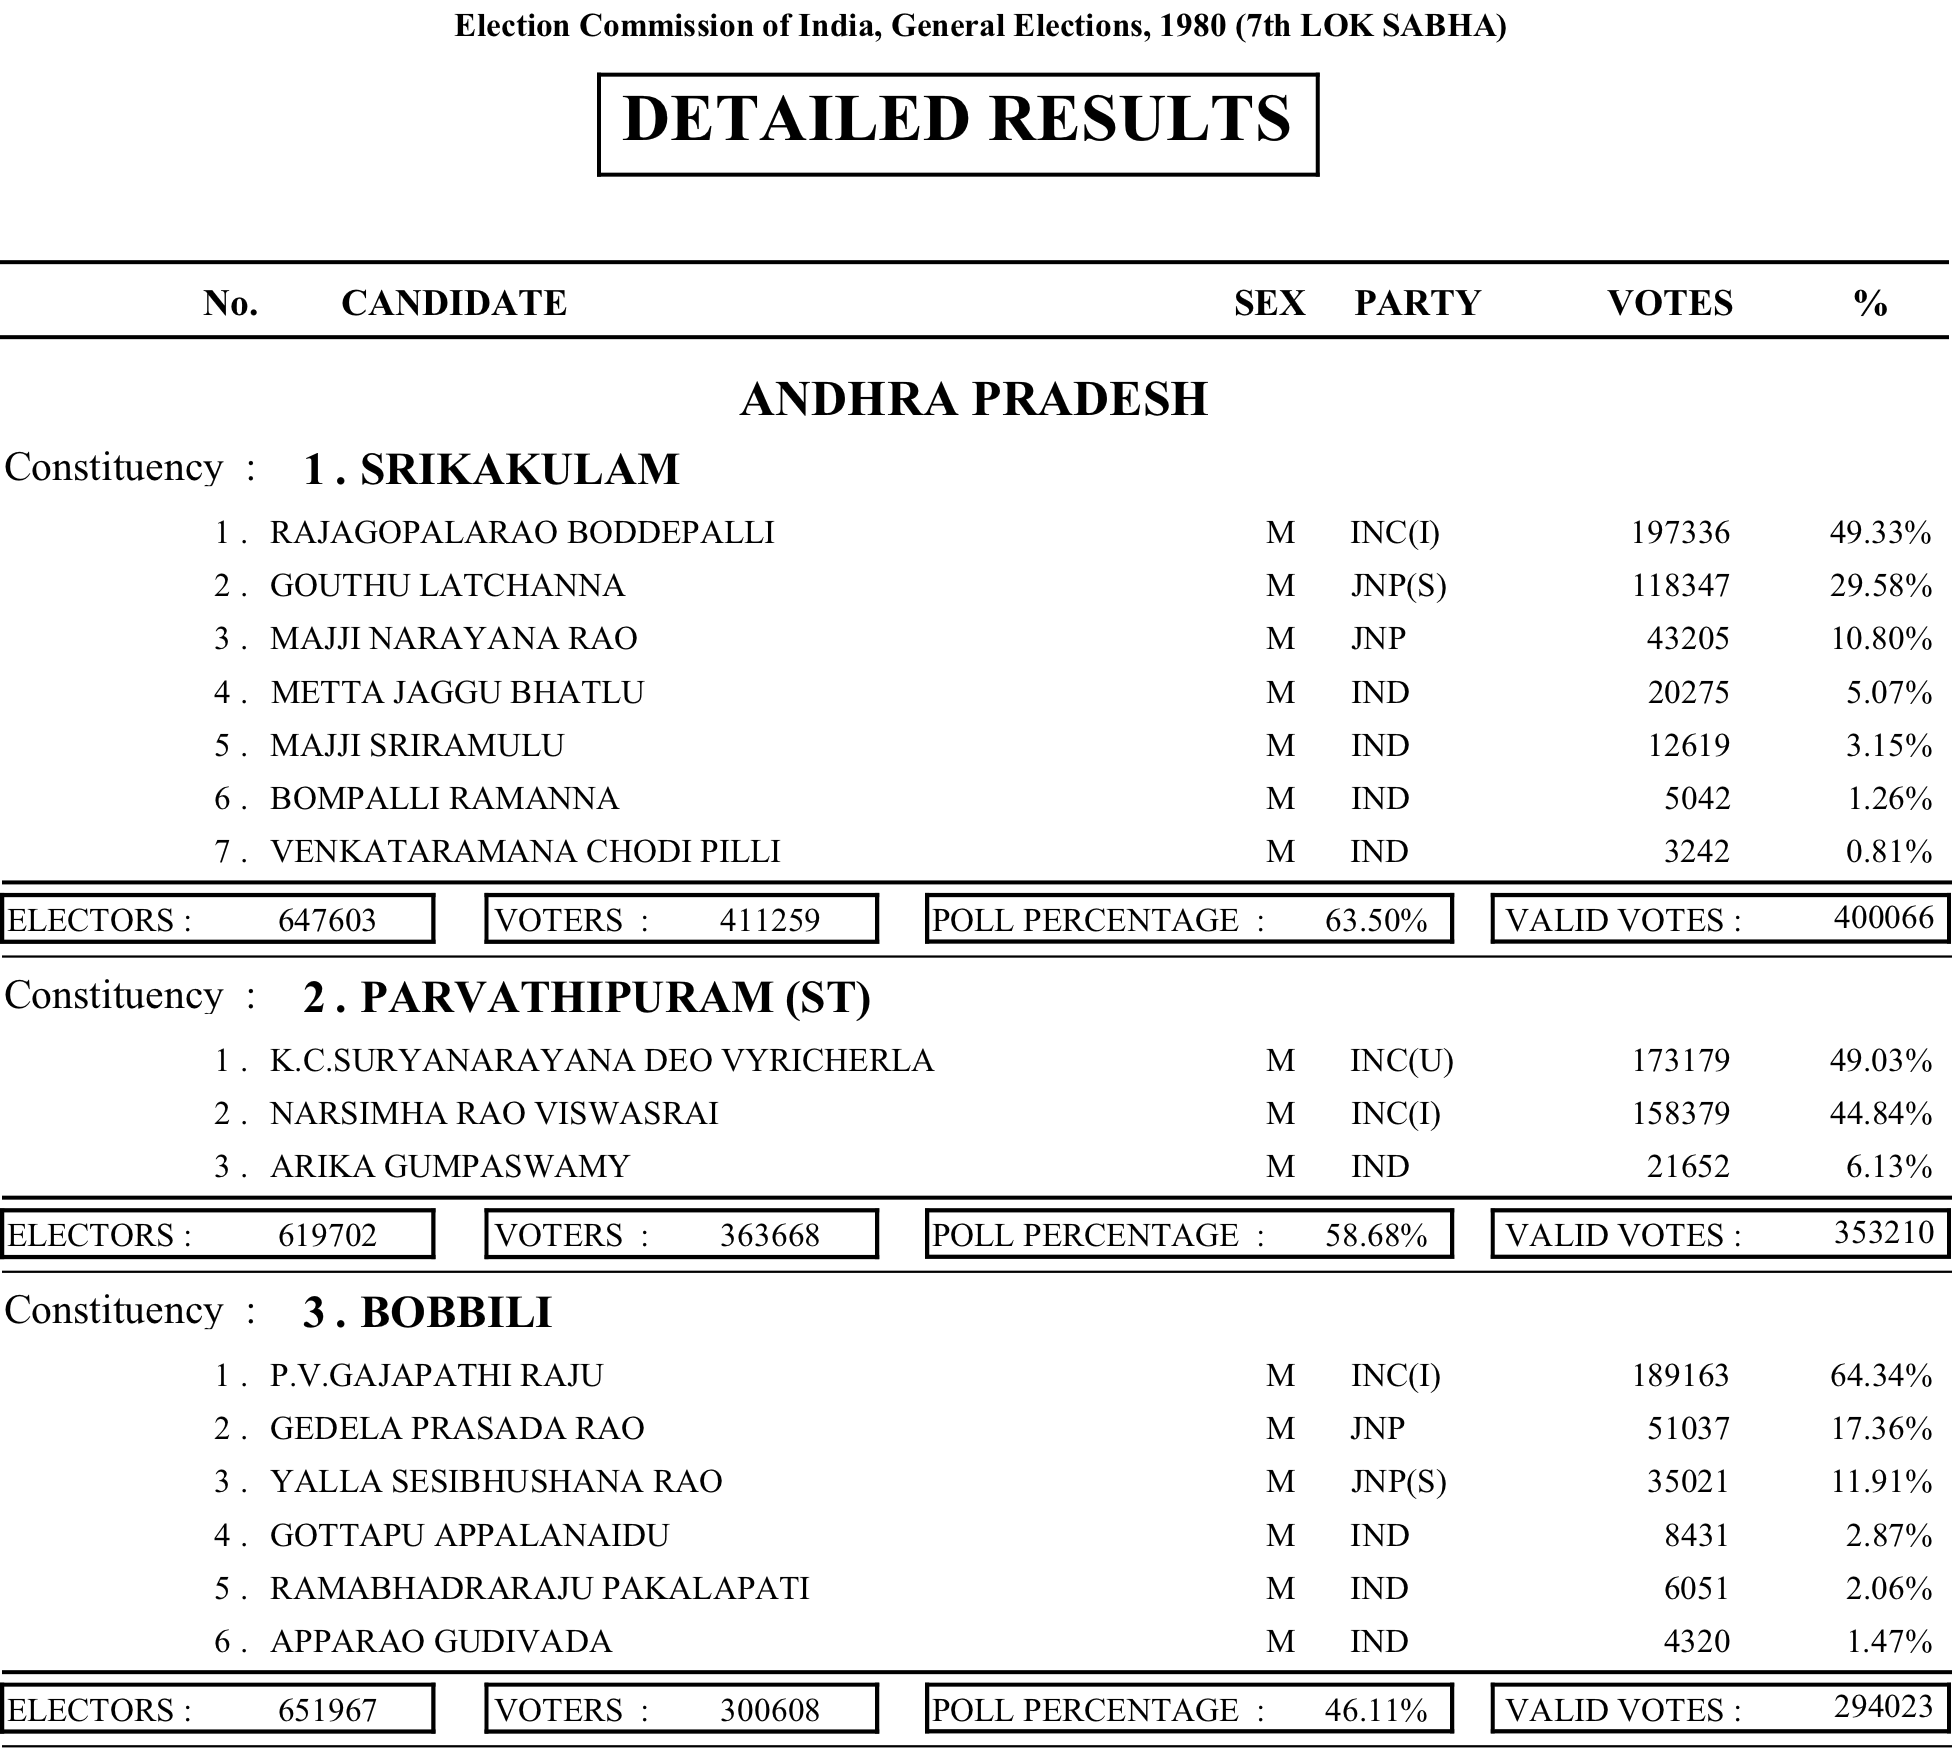
\includegraphics[width=\linewidth]{LS7_DR.png}
  \caption{The Detailed Results section of the statistical report of the 1980 parliamentary elections. The format drifts over time; different reports have different variants of this format.}
%%  \Description{Statistical Report Detailed Results}
  \label{DetailedResults}
\end{figure}


\begin{figure}[h!]
  \centering
  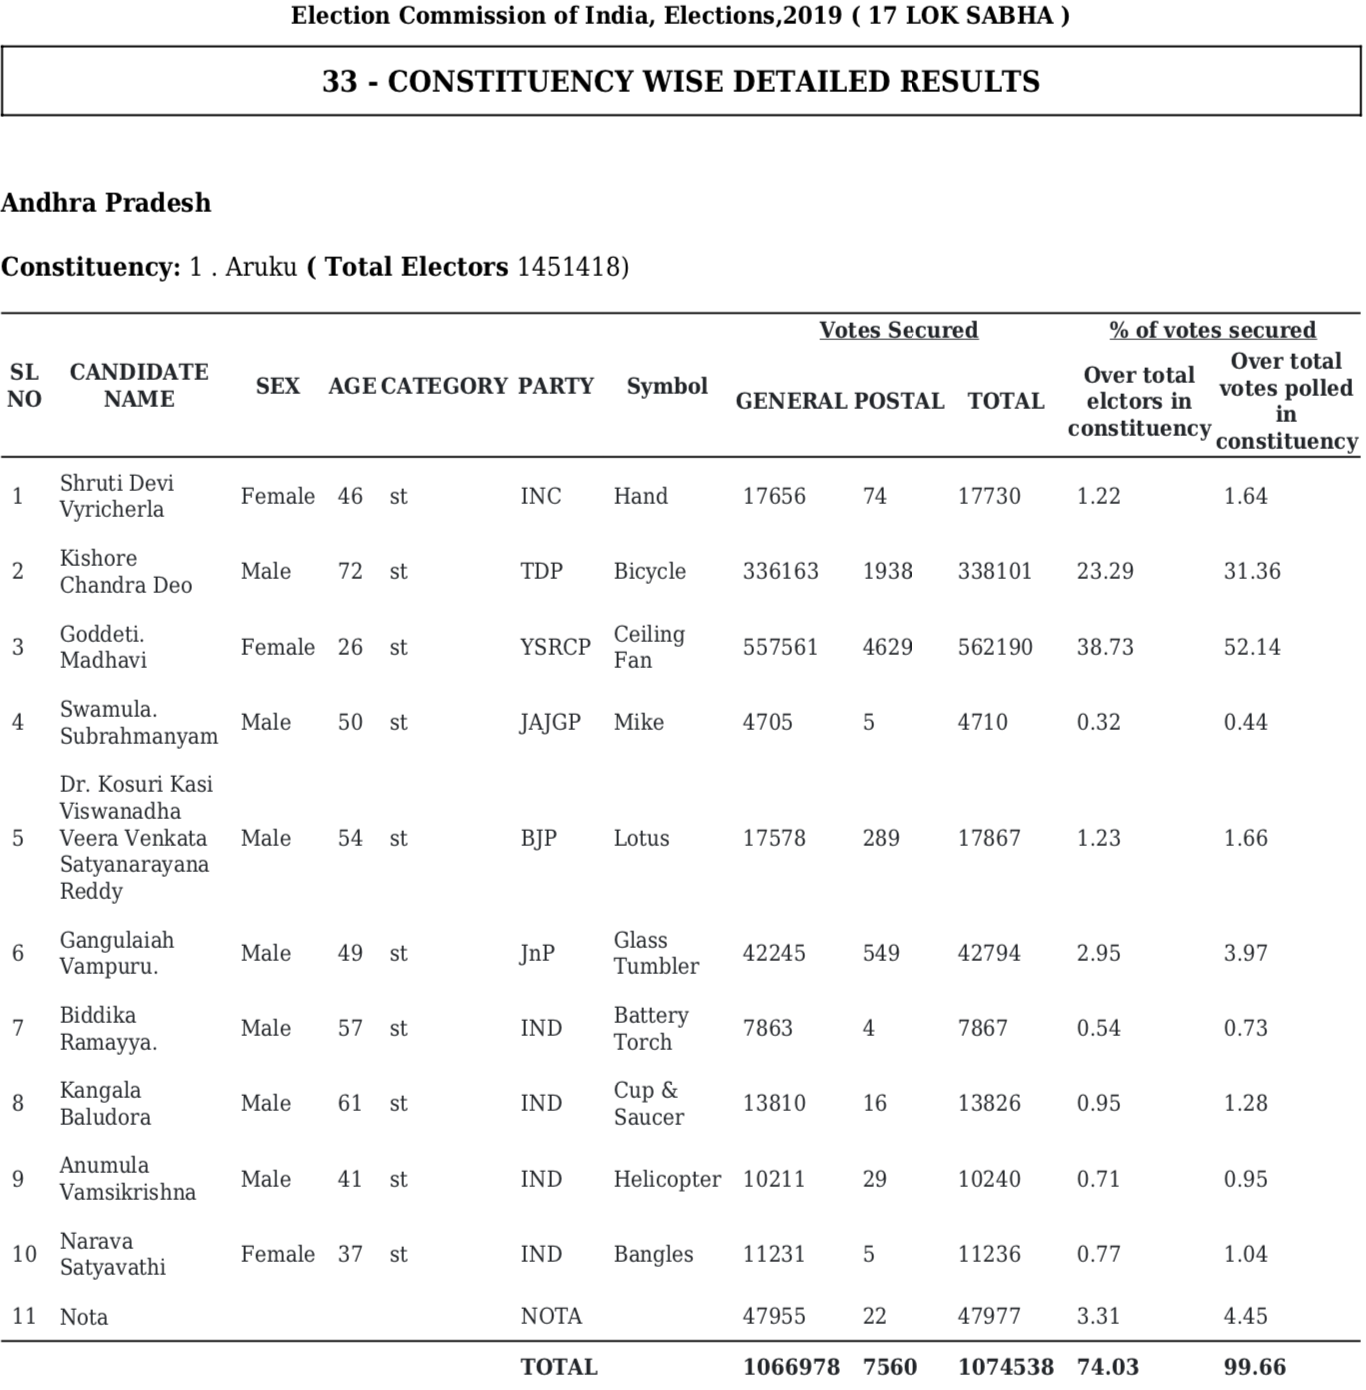
\includegraphics[width=\linewidth]{LS17_DR.png}
  \caption{The Detailed Results section of the statistical report of the 2019 parliamentary elections.}
%%  \Description{Statistical Report Detailed Results}
  \label{DetailedResults17}
\end{figure}
% Some constituencies in India are reserved for Scheduled Castes (SC) and Scheduled Tribes (ST); only candidates from the respective category can contest in them. 

\subsection{Format Drift}

As is often the case with longitudinal data, the formats in these statistical reports have drifted considerably over time. Entire sections have appeared or disappeared in different years; data sections within a page have moved relative to each other, or new fields have got introduced. Figs.~\ref{DetailedResults} and \ref{DetailedResults17}  show the change in format between the 1980 and 2019 statistical reports.

Sections of the source reports often duplicate information, which can lead to inconsistencies. (In database terms, they are non-normalized.) For examples, candidates marked as women in one section of the report may be inconsistently marked as men in another section.

There is also inherent complexity in the data, which needs to be resolved manually. For example, periodic reorganization of Indian states has led to renaming existing states or the creation of new states. These issues can only be tracked manually; LokDhaba handles this by keeping a small set of mapping files to capture this information.

%%The scraped data from general and bye-poll elections is structured as observation variable tables for candidates and constituencies. Each observation for a constituency denotes a contest for a seat in any assembly (state level or parliamentary), and each observation for candidate denotes a candidate who contested any election. The variables capture the information extracted for each observation, which include but not limited to \emph{election type, assembly no, state name, constituency no, poll no, candidate, party, votes}. 
 
\subsection{Data Extraction and Parsing Pipeline}

To design a database for systematically collecting, analyzing and expanding the data on Indian elections, we first needed to extract information about constituencies and candidates from all the statistical reports. The constituency-wise detailed results section contains the electoral information about all the candidates in a given constituency. We build the primary data about candidates by extracting and parsing this section from 342 statistical reports corresponding to all the elections held since 1962. (Elections in prior years had complicated rules like multiple winners in a constituency, making it difficult for our schema to cover them consistently.) 

The structure of this results section varies across the statistical reports in terms of table format and the information present in those tables. Our high-level pipeline to extract, clean and parse this data is shown in Fig. \ref{fig:extraction-pipeline}. This pipeline can be broadly divided into following stages. 
\begin{figure}[h!]
  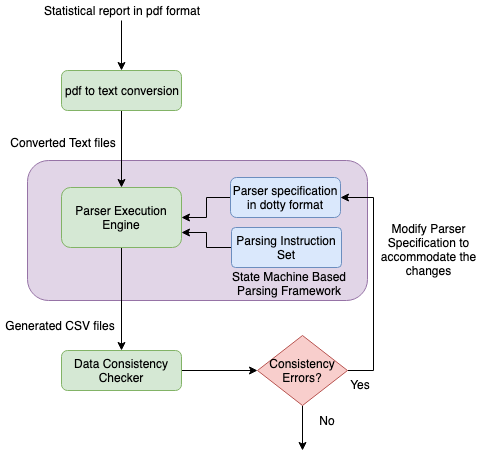
\includegraphics[scale=0.5]{ExtractionPipeline.png}
  \caption{Electoral data extraction pipeline}
  \label{fig:extraction-pipeline}
\end{figure}

\subsubsection{PDF to text conversion} The first step is to use PDF-to-text conversion tools (or optical character recognition tools in some cases) to extract text from the PDF file. If the PDF file was created manually, instead of scanning a paper file, the {\it pdftotext} utility~\cite{pdftotext} gives good results and preserves the layout of the PDF during conversion.

\begin{figure*}
\begin{minipage}{\textwidth}
  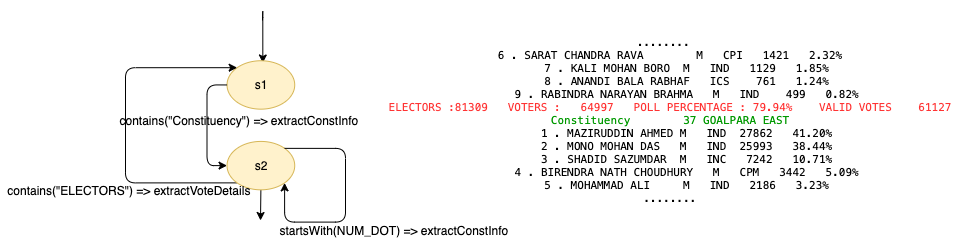
\includegraphics[scale=0.5]{sm-spec.png}
\end{minipage}
\caption{Sample parsing specification program and associated file to parse}
  \label{fig:sample-sm-spec}
\end{figure*}

\subsubsection{Handling format drift} After converting the PDF file to text, we need to parse the text to extract the data in appropriate columns of a structured format. For this purpose, we initially started by developing custom parsers written in the Python programming language. This needed to be done for 342 separate files across all elections. However, the format drift in the tabular structure of these files makes the job of the parser very difficult. Our parser needed a lot of special case handling to handle format mismatches and this was not a solution that would scale and be maintainable in the long run. We have observed that this is a recurrent problem in longitudinal datasets, and therefore it needs a generalizable solution.

Our overall goal is to develop a family of parsers for a set of related formats, in this case, related to Indian elections data. To enable this, we have to come up with a set of parsing rules that are closely tied to the domain and can be easily provided or vetted by domain experts. It is not known how many different parsing specifications will be needed; hence, the specifications themselves need to be iteratively developed as we discover their limitations. In order to detect parsing failures, we need to incorporate a series of consistency checks that pro-actively warn us of such failures, and allow us to develop new specifications or modify existing ones. Consistency checks may be simple (a value in a certain column must be of a certain type) or compound (the values in two columns must satisfy a certain relationship).

Our parsing framework consists of a simple, textually-specified but graphically-viewable programming language. This language captures the essence of the rules needed to parse the family of input files. To develop these specifications, one can write a few simple python functions, and does not need to know any parser generation tools like lex or yacc. The ability to view the parsing specification graphically makes it easy to understand for domain experts who may not be familiar with programming languages.

%\newcommand{trans}{$\delta$}
%\newcommand{lab}{$\sigma$}

A program in our language is represented as a tuple $\left( S,G,A, \mathcal{L} \right)$.  Here $S$ is a set of parsing states, $G$ is a set of guarding conditions, and $A$ is a set of text processing actions. $\mathcal{L}: S \times G \to S \times A$ is a function that assigns a destination state and action to a source state and a guarding condition. Specifically, $\left(s_1,g_1\right) \to \left(s_2,a_1\right) \in \mathcal{L}$ implies a state transition from $s_1$ to $s_2$ if the guarding condition $g_1$ holds at $s_1$; before completing this transition, the text processing action $a_1$ is applied to the input data at $s_1$.  Every guarding condition in $G$ can be of one of the types shown in Table \ref{tab:guarding}. Further, every text parsing action in $A$ can be of one of the types shown in Table \ref{tab:parsingact}. Both the guarding conditions and the parsing actions are fairly domain-specific, but are easy to develop just once, since they refer to intrinsic properties of the data. Hence, their definitions are relatively stable over time.

\begin{figure}[h]
\begin{tabular}{|c|l|} 
 \hline
 \textbf{Condition} & \textbf{Interpretation} \\\hline
 \textbf{true} & always holds true \\\hline
 \textbf{startsWith(s)} & holds true if the line starts with \textbf{s}  \\\hline 
 \textbf{endsWith(s)} & holds true if the line ends with \textbf{s}  \\\hline
 \textbf{contains(s)} & holds true if the line contains string \textbf{s}\\
 \hline
%  \caption{Guarding conditions of the specification language}
%  \label{tab:guarding}
\end{tabular}
\captionof{table}{Guarding conditions\label{tab:guarding}}
\vspace{0.2mm}
\end{figure}

\begin{figure}[h]
\begin{tabular}{|c|l|c|} 
 \hline
 \textbf{Action} & \textbf{Interpretation}& \textbf{\#Variants} \\\hline
 \textbf{extractCandInfo(s)} & \multicolumn{1}{m{3cm}|}{extracts candidate details like name, gender, age, party from string \textbf{s}} &3 \\\hline 
 \textbf{extractConstInfo(s)} & \multicolumn{1}{m{3cm}|}{extracts constitutency details like constituency type, constituency number from  string  \textbf{s}}  & 2 \\\hline
 \textbf{extractVoteDetails(s)} & \multicolumn{1}{m{3cm}|}{extracts vote information from string \textbf{s}} & 1 \\\hline
 \textbf{extractPartyInfo(s)} & \multicolumn{1}{m{3cm}|}{extracts party information like party acronym, full name, party type (national or state) from string \textbf{s}} & 2\\\hline
%  \caption{Text parsing actions of the specification language}
%  \label{tab:parsingact}
\end{tabular}
\captionof{table}{Parsing actions\label{tab:parsingact}}

\end{figure}

The set $A$ consists of parsing functions required to extract useful information from a line of text. For example, the \textbf{extractCandInfo} action specifies that the parser is on the verge of extracting candidate demographic information like name, age, and gender from the upcoming text. The third column of Table \ref{tab:parsingact} represents the number of different variations of each parsing method to cover format drift across different input files. One example of this drift is a rearrangement of the order of fields in candidate information. In some files the candidate's information follows the order of name, age, gender, party, valid votes and total votes. In other files, the order of these fields or the number of fields changed. Due to these issues we created different variants of parsing functions. In all, just 8 parsing actions of four representative methods (\textbf{extractCandInfo}, \textbf{extractConstInfo}, \textbf{extractVoteDetails} and \textbf{extractPartyInfos}) were sufficient to cover all the format drift that we saw in 342 files. 

An example program in our specification language is depicted in Figure \ref{fig:sample-sm-spec}. This program is written to parse candidate information from a text file whose snippet is shown on the right. This snippet, taken from an actual ECI input file, shows the regularity in the structure of the content. It shows a set of lines, one for each candidate's information, followed by a line representing aggregate information (in red), and then followed by the start of information of another constituency. The graphically depicted specification on the left side in Fig. \ref{fig:sample-sm-spec} captures this regularity using two states s1 and s2 and the transitions among them. The transition from s1 to s2 captures the fact that after the aggregate result line in the text snippet (in red) we expect the file to contain a line for the information related to another constituency (in green). The label \textbf{contains("Constituency") => extractConstInfo} on this transition triggers a state change from s1 to s2 if the input line contains the string "Constituency". As a result of this transition, the parsing method \textbf{extractConstInfo} extracts the constituency information from the input line. Further, the fact that there are more than one candidates in a constituency and we need to extract candidate information for all of them is captured by a self transition from s2 to itself. It is to be noted that from a given state more than one transitions can be triggered based on the input data. In this scenario the execution of the parser is stopped with detailed information about the input line in that state. This information is then used to write a more precise specification of the parser so as to traverse only unambiguous transitions.

This specification is passed to a Parser Execution Engine as shown in Fig. \ref{fig:extraction-pipeline}. 
This engine takes a text file as an input and executes the parser specifications to generate a structured database file. Using this approach, we were able to cover the parsing of 342 files by 20 different parser specifications.

\subsubsection{Detecting parsing errors} An important step after getting parsed values from the parsing stage is to perform sanity checks on them. Errors can get introduced at any of the previous stages of the extraction pipeline. For example, PDF to text conversion may not be accurate. Or the parsing phase may wrongly assign the value of one column to another. During our initial development, it was not unusual that a column like, say, `Gender'  would wrongly get mapped into the `Total Votes' column. To detect such anomalies easily and refine our parser, we developed a consistency checking framework. This framework allows domain specialists to express sanity checks for the data in a simple and expressive manner. For example, a person working with electoral data can specify that the number of total votes polled in a constituency should be the sum total of all the votes polled in that constituency by individual candidates. Consistency checks could also be applied to the type of values in a column (a `Gender' column can only contain the values `M', `F', or `O', a `Votes' column can only be a number greater than or equal to 0), or specify constraints between columns. Any violation of such a check indicates a data error has been introduced, and prompts the user to refine the specification or look closely at the source data.

Of course, some of these errors also represent an actual problem in the source data and may require further analysis by a domain expert. Some examples anomalies we observed in our source data were changing of the type of a constituency within a delimitation (which is not expected; see Section \ref{sec:delim}), and more than one candidate from a party contesting in the same constituency.

The consistency checks also helped us to identify special cases in the data that we were unaware of. In constituencies of the Sikkim legislative assembly, we were not aware that the type of a constituency could have the valid tag ``BL'', which marks reservation of the constituency for selected backward classes. We were also able to find out missing results for constituencies. For example, the statistical report for the 7th Parliamentary assembly has data for only 2 constituencies in Assam instead of the expected 10. Similarly, results for \emph{Purnea} constituency in Bihar were missing. Also, comparing total voters to electors in a constituency, as total electors have to be greater than total voters, helped us narrow down errors due to scraping misalignment. The data type checks helped us to identify  missing and incorrect values in bye-elections, missing candidate names in 12 observations, missing votes for a candidate in 56 observations, incorrect constituency or candidate types, and missing gender values in 928 state assembly and 173 national assembly constituencies for 9,104 candidates.

An important objective of our data extraction pipeline is to make the extraction and parsing process as repeatable as possible. This allows us to handle situations when a new version of the data is released, or when better tools become available (say, for OCR) or even when we find a bug in our own tools or processes. Capturing the parsing rules in about 20 high-level directives makes this possible, and is vastly preferable to performing various steps manually.

Our parsing framework can be used in any situation where domain experts and programmers need to work together to convert some source date into a structured format for further processing. It allows non-technical users to effectively take part in the process of data extraction and parsing.


\section{Data Management and Integration}\label{sec:datamanagement}

In this section, we describe how we organize our dataset extracted from the ECI's statistical reports and integrate it with other datasets. The dataset has to be extendable since several new variables are collected by domain experts or field researchers. For example, political scientists often study data across a cohesive sub-region within a state in order to analyze results, trends and swings within such sub-regions. Similarly, they may want to cross-reference this data with data related to administrative units such as districts, and sociological data on candidates such as their caste, religion, and whether they belong to a political dynasty.

\subsection{Structuring Election Results}

The data extracted from ECI statistical reports is stored in relational form, i.e., in several tables, that are almost fully normalized. To support analysts who may need the entire dataset on one screen, scripts are used to stitch the primary tables together and derive a single non-normalized dataset. In order to ensure repeatability in the process, all updates are made only to primary files (under version control), and all derived files are generated only from scripts.

\subsection{Primary and Derived Data}

We now describe the schema of our primary tables. The \textbf{candidates electoral info} table has candidate variables like \emph{candidate name, sex, party, votes}, and the \textbf{constituency electoral info} table has constituency information like \emph{constituency name , electors, voters}, with the tuple \emph{election type, state name, assembly number, constituency number, poll number} as a foreign key to each other.

Using automated scripts, we also compute derived electoral variables useful in political analysis such as \emph{Valid votes, Turnout percentage, Vote share percentage, Deposit lost, Vote margin, Margin percentage and ENOP\footnote{ENOP is the Effective Number of Parties, a common metric used by political scientists to estimate how healthy the competition is in a democracy}}.

Variables related to each individual's political career like \emph{Number of times contested, Number of times won, Previous party, Last Constituency, Whether incumbent/turncoat/re-contesting} are calculated with the help of the candidate's unique identifier, as described in Section~\ref{name_mapping} below.

\subsection{Fragmented Elections and Bye-elections}

While people intuitively associate elections with a specific year (e.g. the 1991 national elections, the 1996 state elections, etc.). the year can be a misleading way of relating sets of elections. For example, the 1991 national elections in India were not conducted in one state (Punjab) due to law and order reasons; elections in Punjab to the same parliamentary House were actually conducted in 1992. Further, in the Indian election system, a bye-election is called when a seat becomes vacant due to death, resignation or disqualification of an incumbent. This bye-election election data is provided separately by the ECI and is released separately from the statistical reports\cite{bipolls}. Bye-election data until 1995 is available as a single spreadsheet with multiple worksheets for national and state elections \cite{bipolls52-95}. Results from 1996 to 2008 are released as HTML pages, and results from 2009 onward are released as Microsoft Excel files with results for each constituency in different worksheets. Once again, we see the presence of format drift. As a result of the difficulty of dealing with disparate formats, bye-election data is rarely factored into political analyses. However, for the purpose of calculating important metrics related to incumbency (the number of sitting members who re-contested, and were elected or lost), it is essential to know the sitting members at the end of an assembly's term, and therefore, to handle bye-election data.

To handle all these cases and merge them into a single table with a consistent schema in LokDhaba, we associate sets of elections with assembly (i.e., legislative house) numbers instead of years. Therefore a particular election in a particular constituency is identified by a tuple of (``Assembly Number'', ``State Name'', ``Constituency Number'' and ``Poll Number''). The variable ``Poll Number`` is used to accurately record bye-elections data. Increasing Poll Numbers represent successive elections for a seat in a given assembly.

\subsection{Unique Identifiers for Names}

Many political science questions require identifying the trajectory of entities such as parties, candidates and constituencies over time. This needs us to be able to assign unique identifiers to these entities, when none exist in our source data.

\subsubsection{Election Candidates}
\label{name_mapping}
To be able to study the career trajectory of every individual candidate, we need a unique identifier for each person across time -- something that the source datasets do not include. This is a complex task because the spelling of the \emph{Candidate Name} field in the dataset can be the same for two different individuals and can be different over time for the same individual. Candidates switch parties and constituencies between elections and it is not possible to use the existing set of variables to make a unique identifier for any single individual. For this reason, a human-in-the-loop entity mapping and resolution system for Indian names called Surf \cite{Surf} was designed and implemented to assign a unique identifier for each individual candidate. Surf clusters records based on a resolution variable, which is \emph{Candidate Name} in the current context, based on a similarity metric designed specifically for Indian names. It handles phonetic matching, edit distance based clustering, expected variations like initialization of first and middle names, and expected streaks of candidates contesting consecutive elections. Initially, each record in the dataset is given a unique ID and functionality to merge records within or across clusters is implemented in the interface. A human analyst merges or unmerges records based on her knowledge, along with secondary research on every candidate and constituency. Surf's user interface makes certain operations in this research easier, such as mapping place names and searching for news about a candidate. This work has helped us create a unique identifier for every candidate who has contested any election in the dataset.

\subsubsection{Political Parties}

A similar problem is that statistical reports often use abbreviations to indicate a candidate's party. However, the abbreviations given to parties in the source dataset across elections are inconsistent, making it difficult to track party performance over time. The same parties have been assigned multiple abbreviations, for example, Bharatiya Janata Dal (BHJD, BAJD, BajD, BhJD), Aam Aadmi Party (AAAP, AAP), All India Anna Dravida Munnetra Kazhagam (ADK, ADMK, AIADMK, AIDMK), Indian National Congress (CONG, INC, INC(I), CON) and so on, for over 300 parties. The same abbreviation is also given to two different parties ad different times, for example AAP (Aam Aadmi Party, Awami Aamjan Party), BJS (Bharatiya Jan Sabha, Bharatiya Jana Sangh, Akhil Bharatiya Jana Sangh). Considering the inaccuracies this could lead to in aggregating party-wise data, we assign a unique identifier for each party using the same technique used for resolving names described in the previous section \cite{nissa2019party, nissa2019factions}.

\subsubsection{Electoral Constituencies}
\label{sec:delim}

In India, a Delimitation Commission periodically reorganizes boundaries of electoral constituencies to account for changes in population as measured by the decadal Census of India. Four major delimitations have been made so far, in 1952, 1962, 1972 and 2002, along with amendments in 2001, 2003 and 2008. In each delimitation, two thirds of the constituencies for a state are reorganized. This also means a reassignment of constituency numbers and names. As such, there is no authoritative way to map constituencies across delimitations. As described later, this requires us to assign a unique identifier for each constituency to analyse spatial characteristics with respect to an older time period.

% Public domain constituency maps are available only for the last delimitation in 2008. 

% \subsection{Keeping data updated}
% Elections to the states in India are spread such that every 6 months or so there is an election for at least two states. With each election since 2004, contesting candidates are required to release affidavits. From the affidavit archive, we scrape constituency, candidate and party for all contesting candidates. A working dataset is then created to extract \emph{pid, party id, sociological profile}, for each contesting candidate.

\subsection{Integration with Other Datasets}

% \subsubsection{Sociological data}
% TCPD is also collecting data on sub-castes, caste, religion and political families of candidates from major parties. This data is managed as an independent candidate level primary file having constituency level variables as well, so it can be treated as a separate dataset to collect and update sociological profiles of candidates and elected representatives.

\subsubsection{Affidavit Data}
Beginning in 2004, it is mandatory for every election candidate in India to file an affidavit declaring information such as their address, education, profession, spouse, criminal cases and financial assets. This data is digitized by the Association of Democratic Reforms (ADR) and is disseminated on their website \cite{myneta}. We scrape this data and integrate it with the elections dataset. After resolving inconsistencies in candidate names and parties, new candidate-level primary tables are created with structured fields for this affidavit data.

\subsubsection{Pictures}
In order to aid visualizations of candidate performance, we use the pictures of electoral winners that are available from the website of PRS Legislative Research, a think-tank that tracks performance of legislators. See Fig.~\ref{incm_rhl} for an example of how these pictures are used. 

\subsection{Maps}

In this section, we describe some of the challenges of dealing with geo-spatial data, required for map visualizations built upon our dataset. In India, state-level constituencies are properly nested and contained within national constituencies. The present constituency boundaries at both levels were specified in the 2008 delimitation. Unfortunately, official spatial boundaries are not made available in digital format by the delimitation commission. A group called Datameet has developed a novel solution to this problem -- it scraped the GPS locations of the polling stations in the 2014 election, and derived approximate constituency boundary maps based on this data~\cite{datameet}. We adopted these maps as a starting point and applied consistency checking to detect potential problems. 

There are a total of 543 national-level and 4120 state-level constituencies. We identified inconsistencies by comparing each constituency on area, neighbourhood and mapping of state-level constituencies to the national-level constituency they were contained in. This process helped us find problems with incorrect borders or missing constituencies in the original maps. We cross-referenced boundary polygons from the Datameet maps with constituency-wise listings from election results. We observed that a few urban constituencies were missing. Consistency checks on the area of each constituency also helped us identify some constituencies with suspiciously low area, for example, less that one square kilometer. For missing or inconsistent constituencies found in the above steps, we derived the correct shapes using manual digitization of the respective sub-districts, villages and municipal wards. The geometries of resulting boundaries are simplified further to remove overlaps and holes between polygons.

\subsection{Data Provenance and Management}

To store data and manage updates to our database, we use a git repository which stores all versions of all primary files and scripts. Data files are stored in CSV format, allowing efficient storage of revisions of the data, and ensuring no lock-in to any proprietary format. Revision control also allows us to track changes down to the time and person responsible for the change, and to roll back to any version if necessary. LokDhaba follows an Engineering Change Order (ECO) process by which each change has to be first vetted by multiple people before it is introduced in the primary dataset. This ensures that the data quality remains fairly high.

LokDhaba has scripts that compute derived data from primary data dynamically. To alert us to any loss in data quality, data consistency checking scripts run nightly as a cron job. The process for extracting data from affidavits and results is also automated using scripts, ensuring that we can re-import data from some source, if and when it changes. This ensures the repeatability of our process. 



\section{Data Dissemination}

In addition to extracing and organizing the dataset, we designed a web application with which a user can browse and visualize the data on-demand. The user can download various versions of the dataset and visualize the political variables spatio-temporally. Keeping scalability and consistent user experience in mind, LokDhaba is implemented with a model-view-controller architecture. The tables described in the previous section are converted into an SQL database that provides the model. This database is exposed through a Python API, and a React-based framework is used for fast rendering of visualizations with client-side filtering.

%The whole system is composed in docker with db, api and react node as independent interlinked services. 

The main ways for an end-user to interact with the data are the following:
\begin{itemize}
    \item \textbf{Browse and Download Data}: the user can explore and download the dataset online.
    \item \textbf{Data Visualization}: the user can build charts and maps to visualize election results from a political science perspective.
    \item \textbf{Incumbency profile}: the user can explore the career performance of election candidates using a novel visualization interface.
\end{itemize}

\subsection{Data Preparation}

The front-end access to LokDhaba is characterized by read-only operations. LokDhaba uses a MySQL database to store and retrieve data efficiently. Pre-computed tables are stored for assembly, constituency, party and candidate level tables to provide quick visualizations in the front-end.

%This database is executed as a separate docker service which gets initialized with empty tables whenever the service is build. This design implementation of database helps keeps us away from managing databases and related issues with security, performance, safety, resource utilization and availability.

An API based on representational state transfer architecture (REST) is implemented in Python as the interface between the React-based front-end and the database. Various pieces of functionality are designed as React ``routes'' to get data for different visualization inputs, constituency boundaries, paginated browsing and download. The API receives inputs from the user interface via POST requests, creates parameterized SQL queries to extract data from the database, and sends it back as JSON objects.  

\subsection{User Interface}

The main components for the user interface are as follows.
 
\subsubsection{Browse and Download Data}
 
 While LokDhaba incorporates several visualizations, it is important to enable users to download the raw or filtered datasets to perform their own analysis. It is also important for users to zoom in to a specific row in the table if they are interested in a particular election, or a particular candidate, etc. The Browse and Download component is designed for viewing, filtering, and sorting raw data for any election. The user selects election type and state name, and multiple assemblies of the selected state to view election results. She can also download raw data, filtered down based on any criteria, as a comma separated values (CSV) file. This component uses a \emph{react-table} component to render a large number of rows as a paginated table. It also supports quick, client-side filtering and sorting.
 
 Fig.~\ref{browse} shows a screenshot of the browse data component with results for the 2019 Parliamentary elections. Note that the position is filtered to 1, so as to list only winning candidates. Users can also filter by any other value on different columns.
  
 \begin{figure}
 \centering
 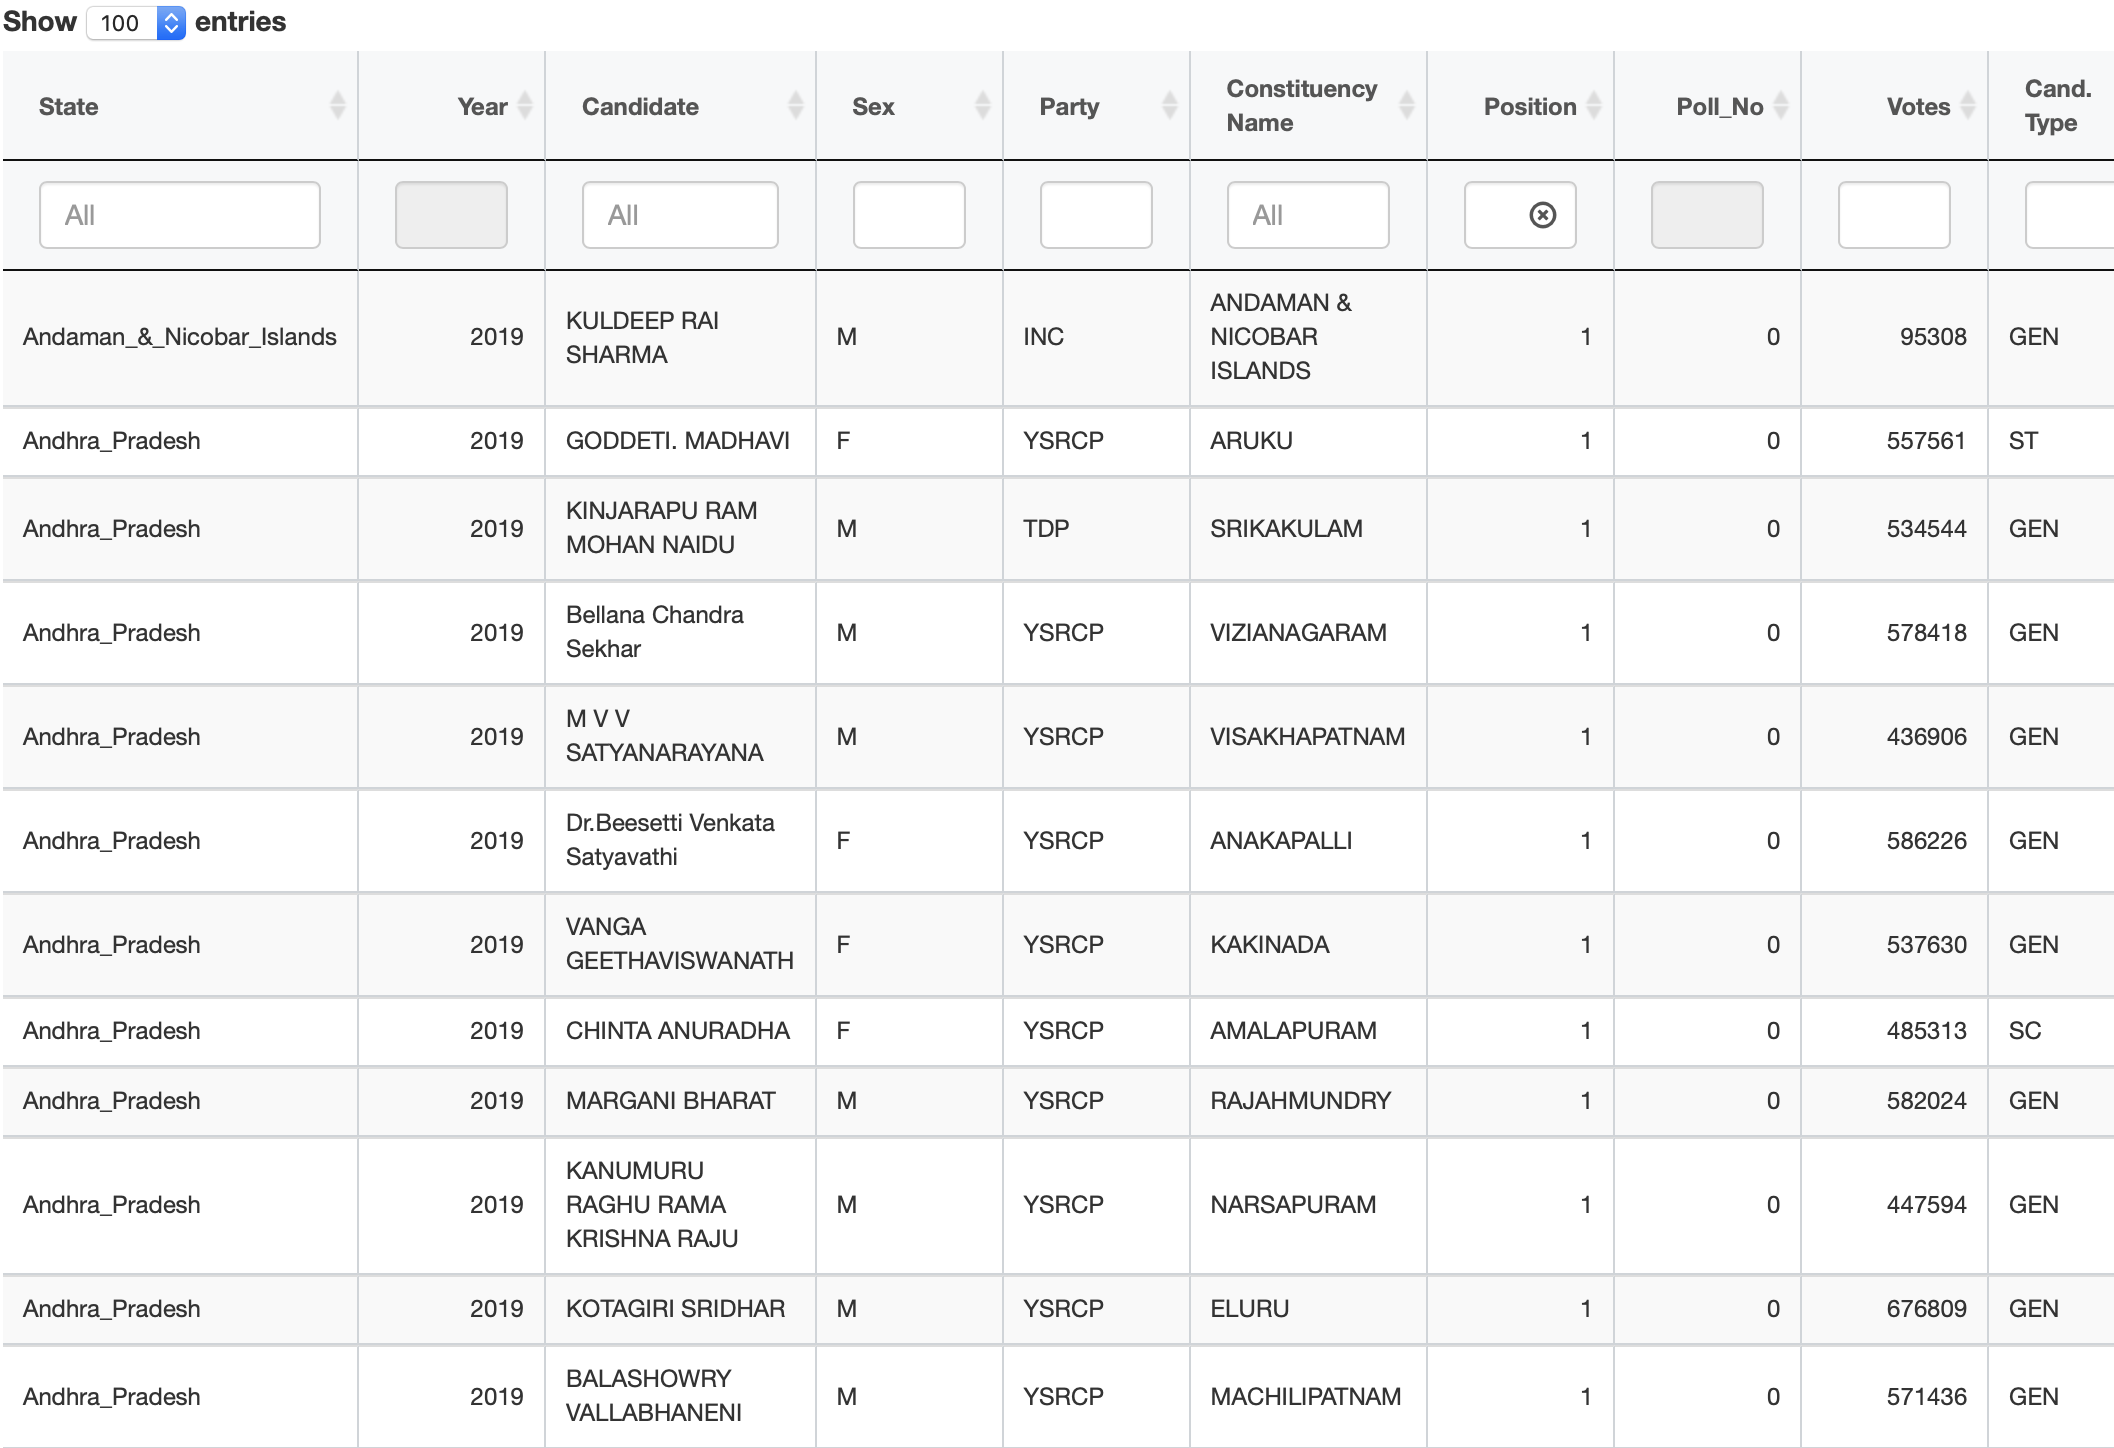
\includegraphics[width=\linewidth]{BrowseLS17Winners}
 \caption{Browse data to show all position 1 candidates of the 2019 Parliamentary election}
%%  \Description{browse ls17 winners}
 \label{browse}
 \end{figure}
 
 \subsubsection{Data Visualization}
  To implement visualizations in LokDhaba, we interviewed political scientists and analyzed media reports to see which visualizations would be the most useful. Based on this analysis, we designed the following time-line charts and visualizations which can be created on-demand by the user for any set of elections.

\begin{enumerate}
    \item \textbf{Voter turnout}: male, female and total voter turnout percentages.
    \item \textbf{Party vote share (contested)}: vote share percentage of main parties for seats they contested. (Not all parties contest all seats, especially in the presence of seat-sharing agreements.)
    \item \textbf{Party vote share (all seats)}: vote share percentage of the main parties across all seats.
    \item \textbf{Party seat share}: seat share percentage of the main parties.
    \item \textbf{Parties contested and represented}: number of parties that contested and number of parties that got at least one candidate elected.
    \item \textbf{Candidates contested/deposit lost}: number of candidates who contested the election and number of candidates who lost their deposits.
\end{enumerate}

To enable spatial exploration of election results, we came up with the following set of maps\footnote {As shape files for pre-2008 elections are not available, the current version of LokDhaba has maps only for elections post-2008.}. The maps fall into two basic categories: heat maps showing the intensity of a variable (e.g., vote share of a party), and categorical maps used to indicate spatial distribution (e.g., winning party across space).

\begin{enumerate}
    \item \textbf{Constituency type}: different colors for constituency type, a field which can be one of (1) General (open for any one to contest), (2) SC (scheduled caste candidates only) or (3) ST (scheduled tribe candidates only).
    \item \textbf{Number of candidates}: a heat map showing number of candidates contesting in each constituency.
    \item \textbf{Voter turnout}: a heat map of the voter turnout percentage in each constituency.
    \item \textbf{Winners by party}: party-wise coloring for the winning party in each constituency. Parties are mapped to color that are naturally associated with them, using a small color mapping file.
    \item \textbf{Winners by gender}: gender-wise coloring for the winner in each constituency.
    \item \textbf{Victory margin}: a heat map of the difference between the winner and first runner-up in each constituency.
    \item \textbf{Vote share of winners}: a heat map of the vote share percentage of the winner in each constituency.
    \item \textbf{Party-wise positions}: a heat map of the rank of the specified party's candidates in each constituency.
    \item \textbf{Party-wise vote share}: a heat map of the vote share percentage of the specified party's candidates in each constituency.
    \item \textbf{NOTA vote}: a heat map of the NOTA (None of the Above) vote share percentage in each constituency.
\end{enumerate}

  The data visualization component is designed to visualize aggregated statistics at a temporal or spatial level. The user selects election type, state name, visualization, and visualization specific variables to be charted or mapped. The individual visualization components take returned data from the API to render charts in \emph{react-plotly} and maps in \emph{react-leaflet}.
 
 Some screenshots of the visualization components are shown in Figs. \ref{partyCR} to \ref{partyWn}. Fig. \ref{partyCR} shows the timeline of parties contested and parties represented over all national assembly assemblies as a bar chart. Fig. \ref{partyVS} shows the vote shares of the ``main'' parties\footnote{Parties in the top two positions by seat share in any previous election.}.

  Figure \ref{BJPVS} shows a heat map of vote shares of candidates from the BJP party in the 17th Parliamentary elections. Fig. \ref{partyWn} shows the constituencies of elected members to the 17th Parliament, color coded by party.
 \begin{figure}
  \centering
  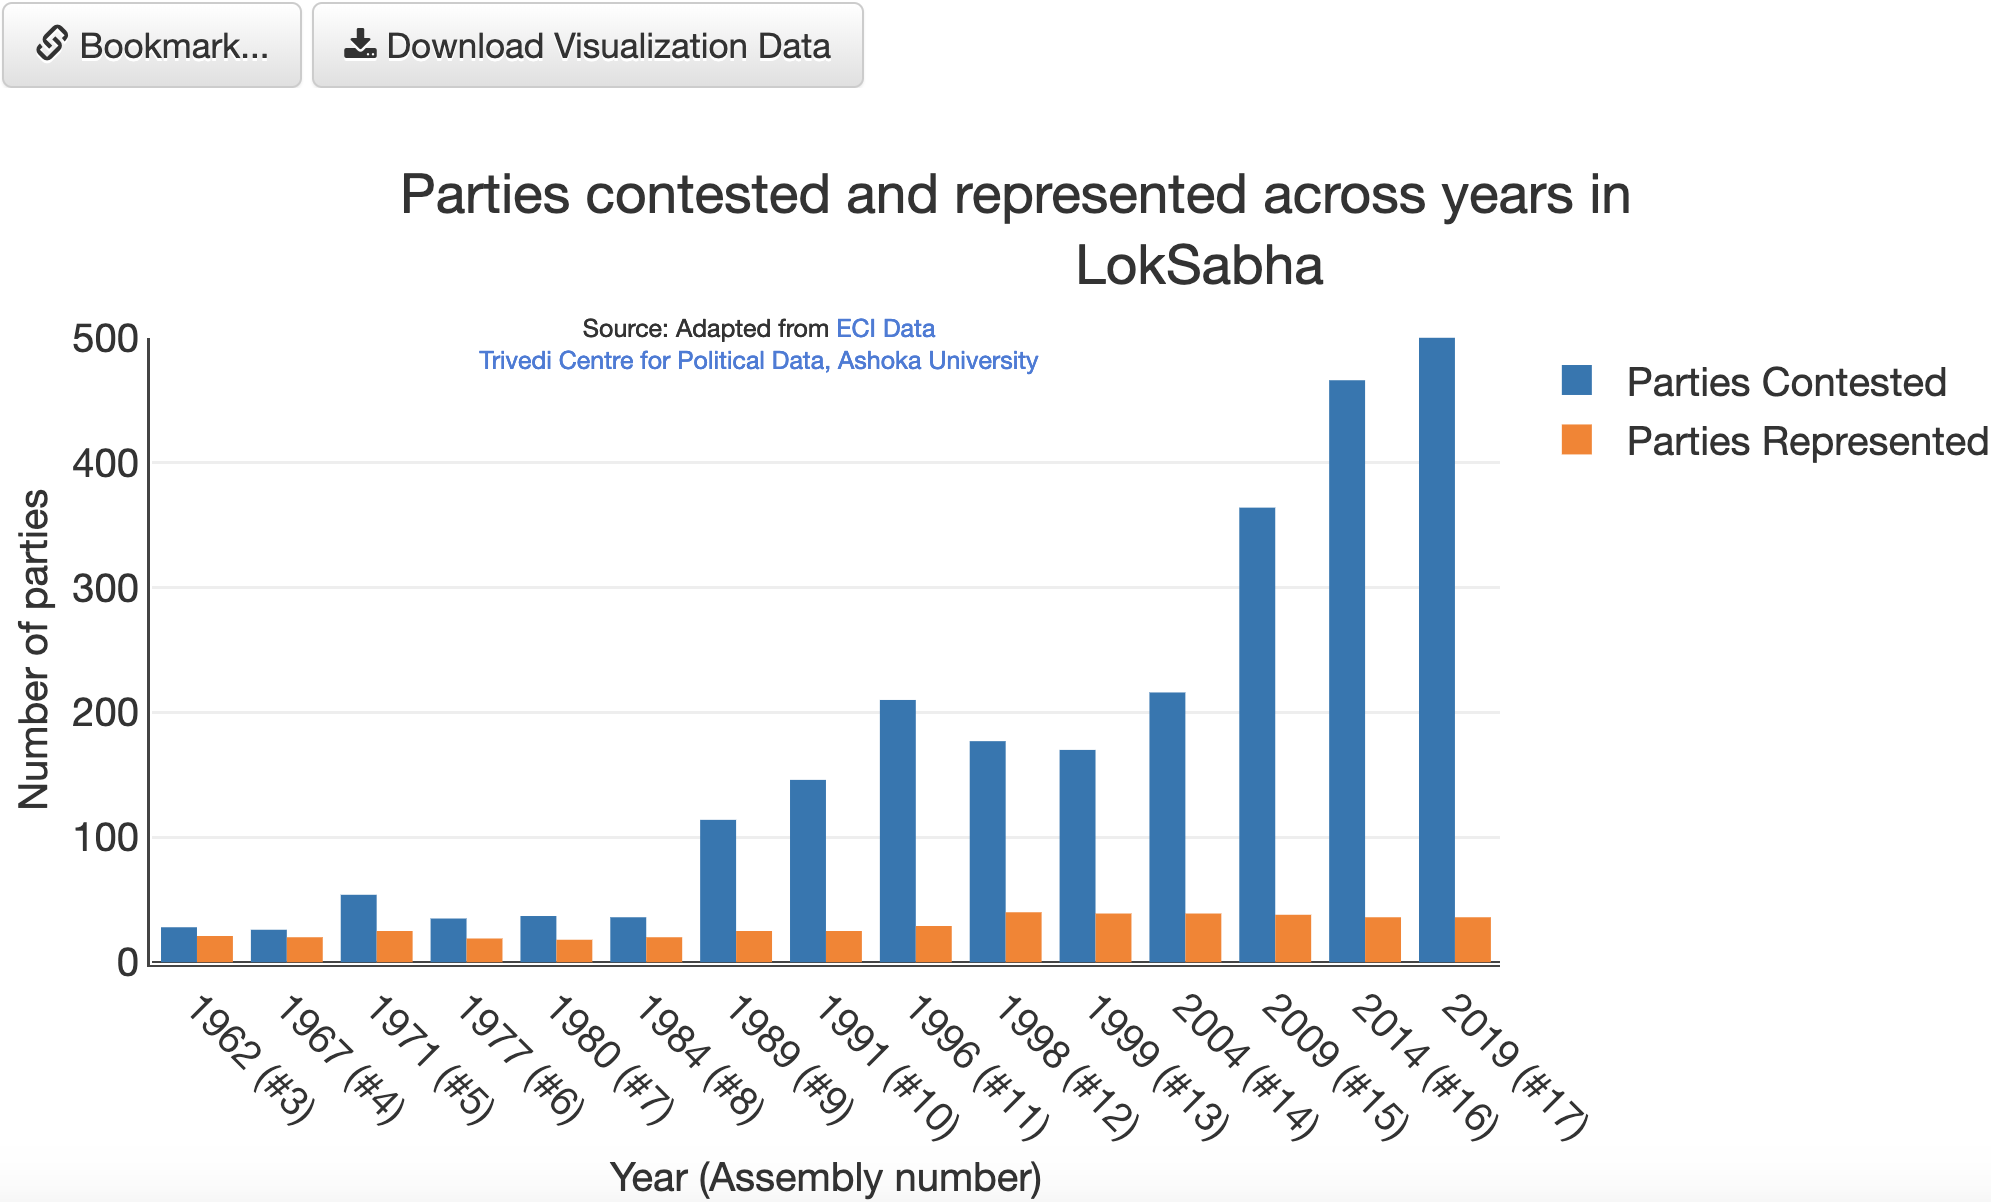
\includegraphics[width=\linewidth]{partiesContestedRepresented}
  \caption{LokDhaba visualization of parties contested and represented in national elections}
  \label{partyCR}
  \end{figure}
  
  \begin{figure}
  \centering
  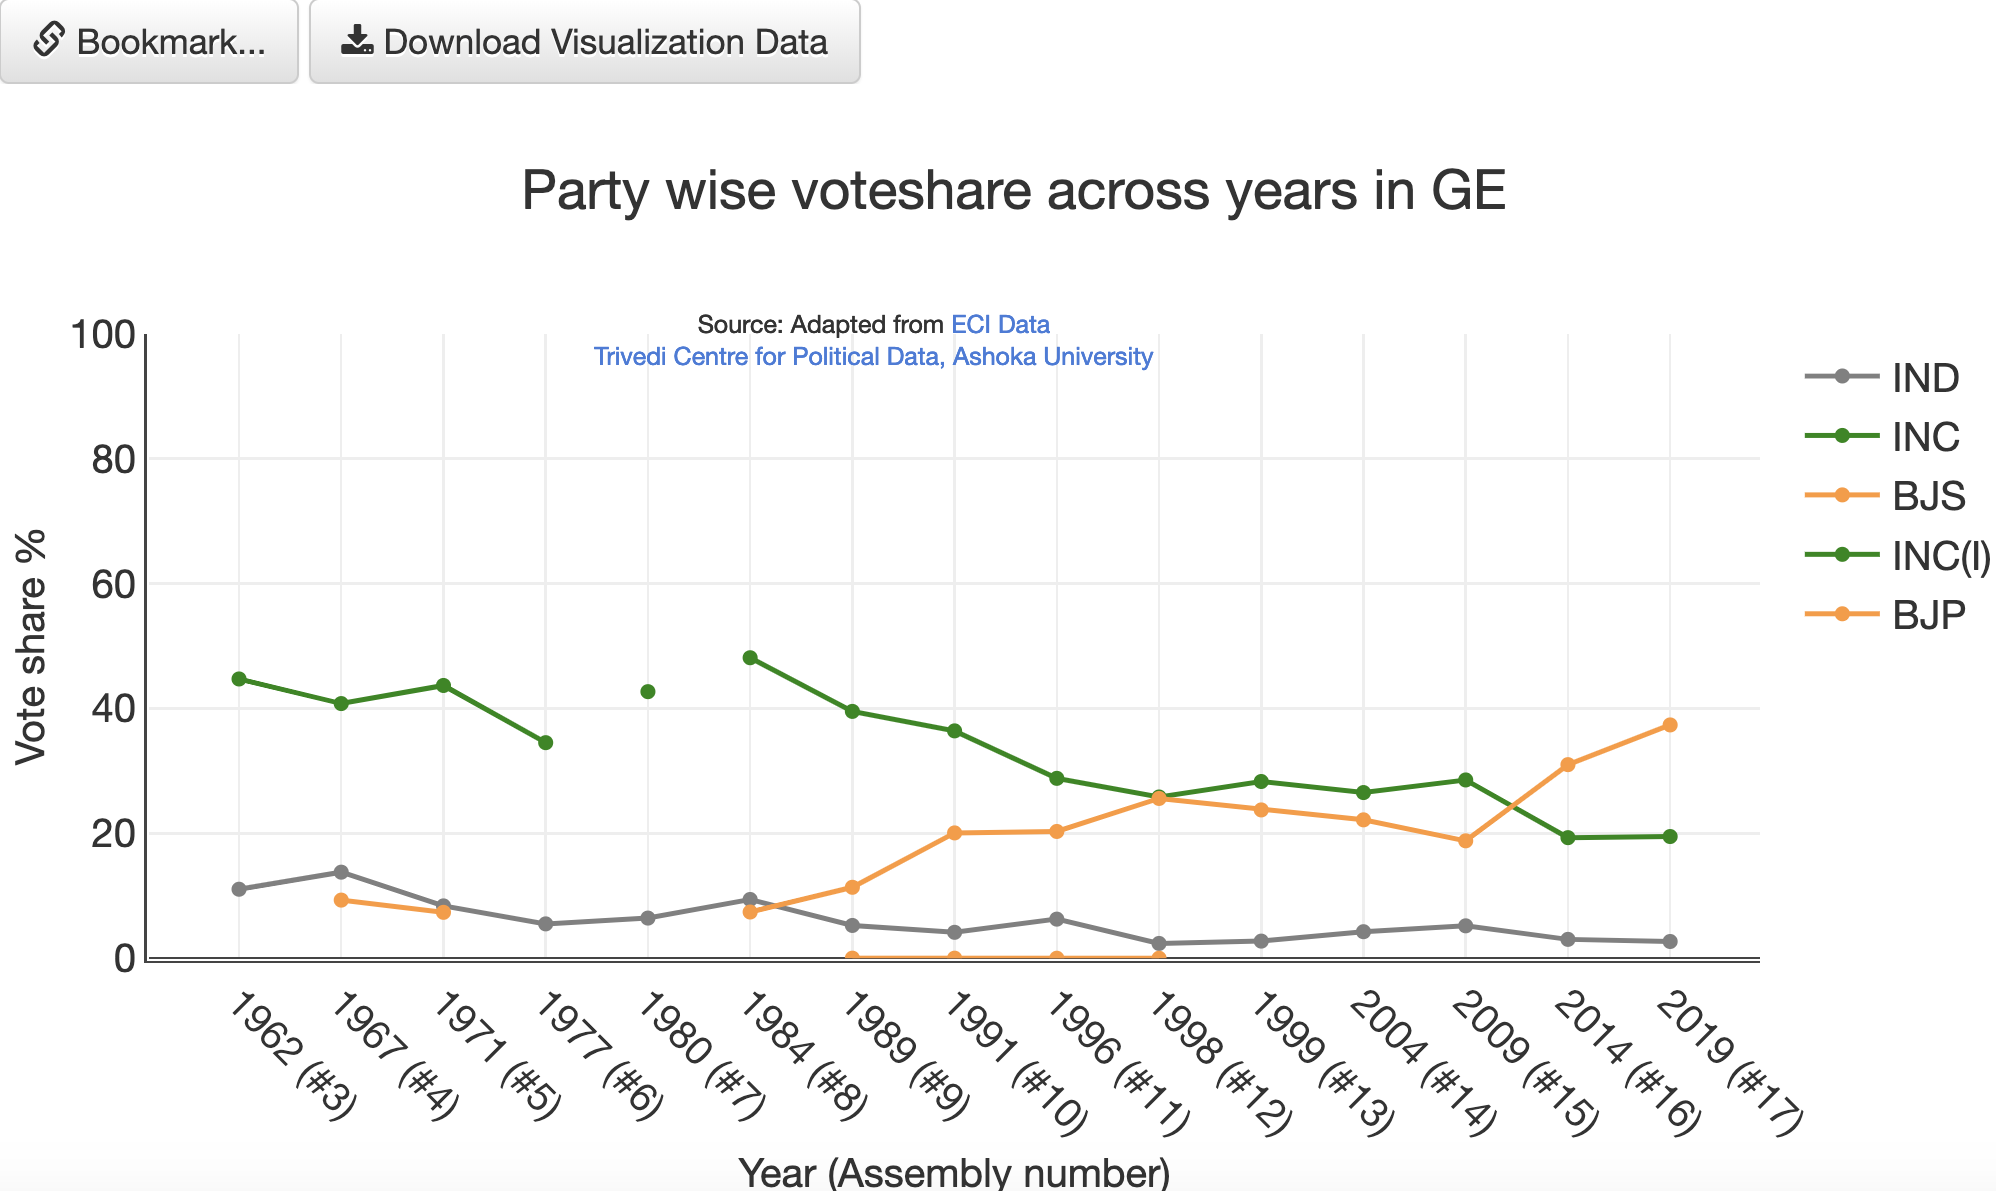
\includegraphics[width=\linewidth]{partyVoteShareTimeline}
  \caption{LokDhaba visualization of party vote shares in national elections}
  \label{partyVS}
  \end{figure}

 \begin{figure}
 \centering
 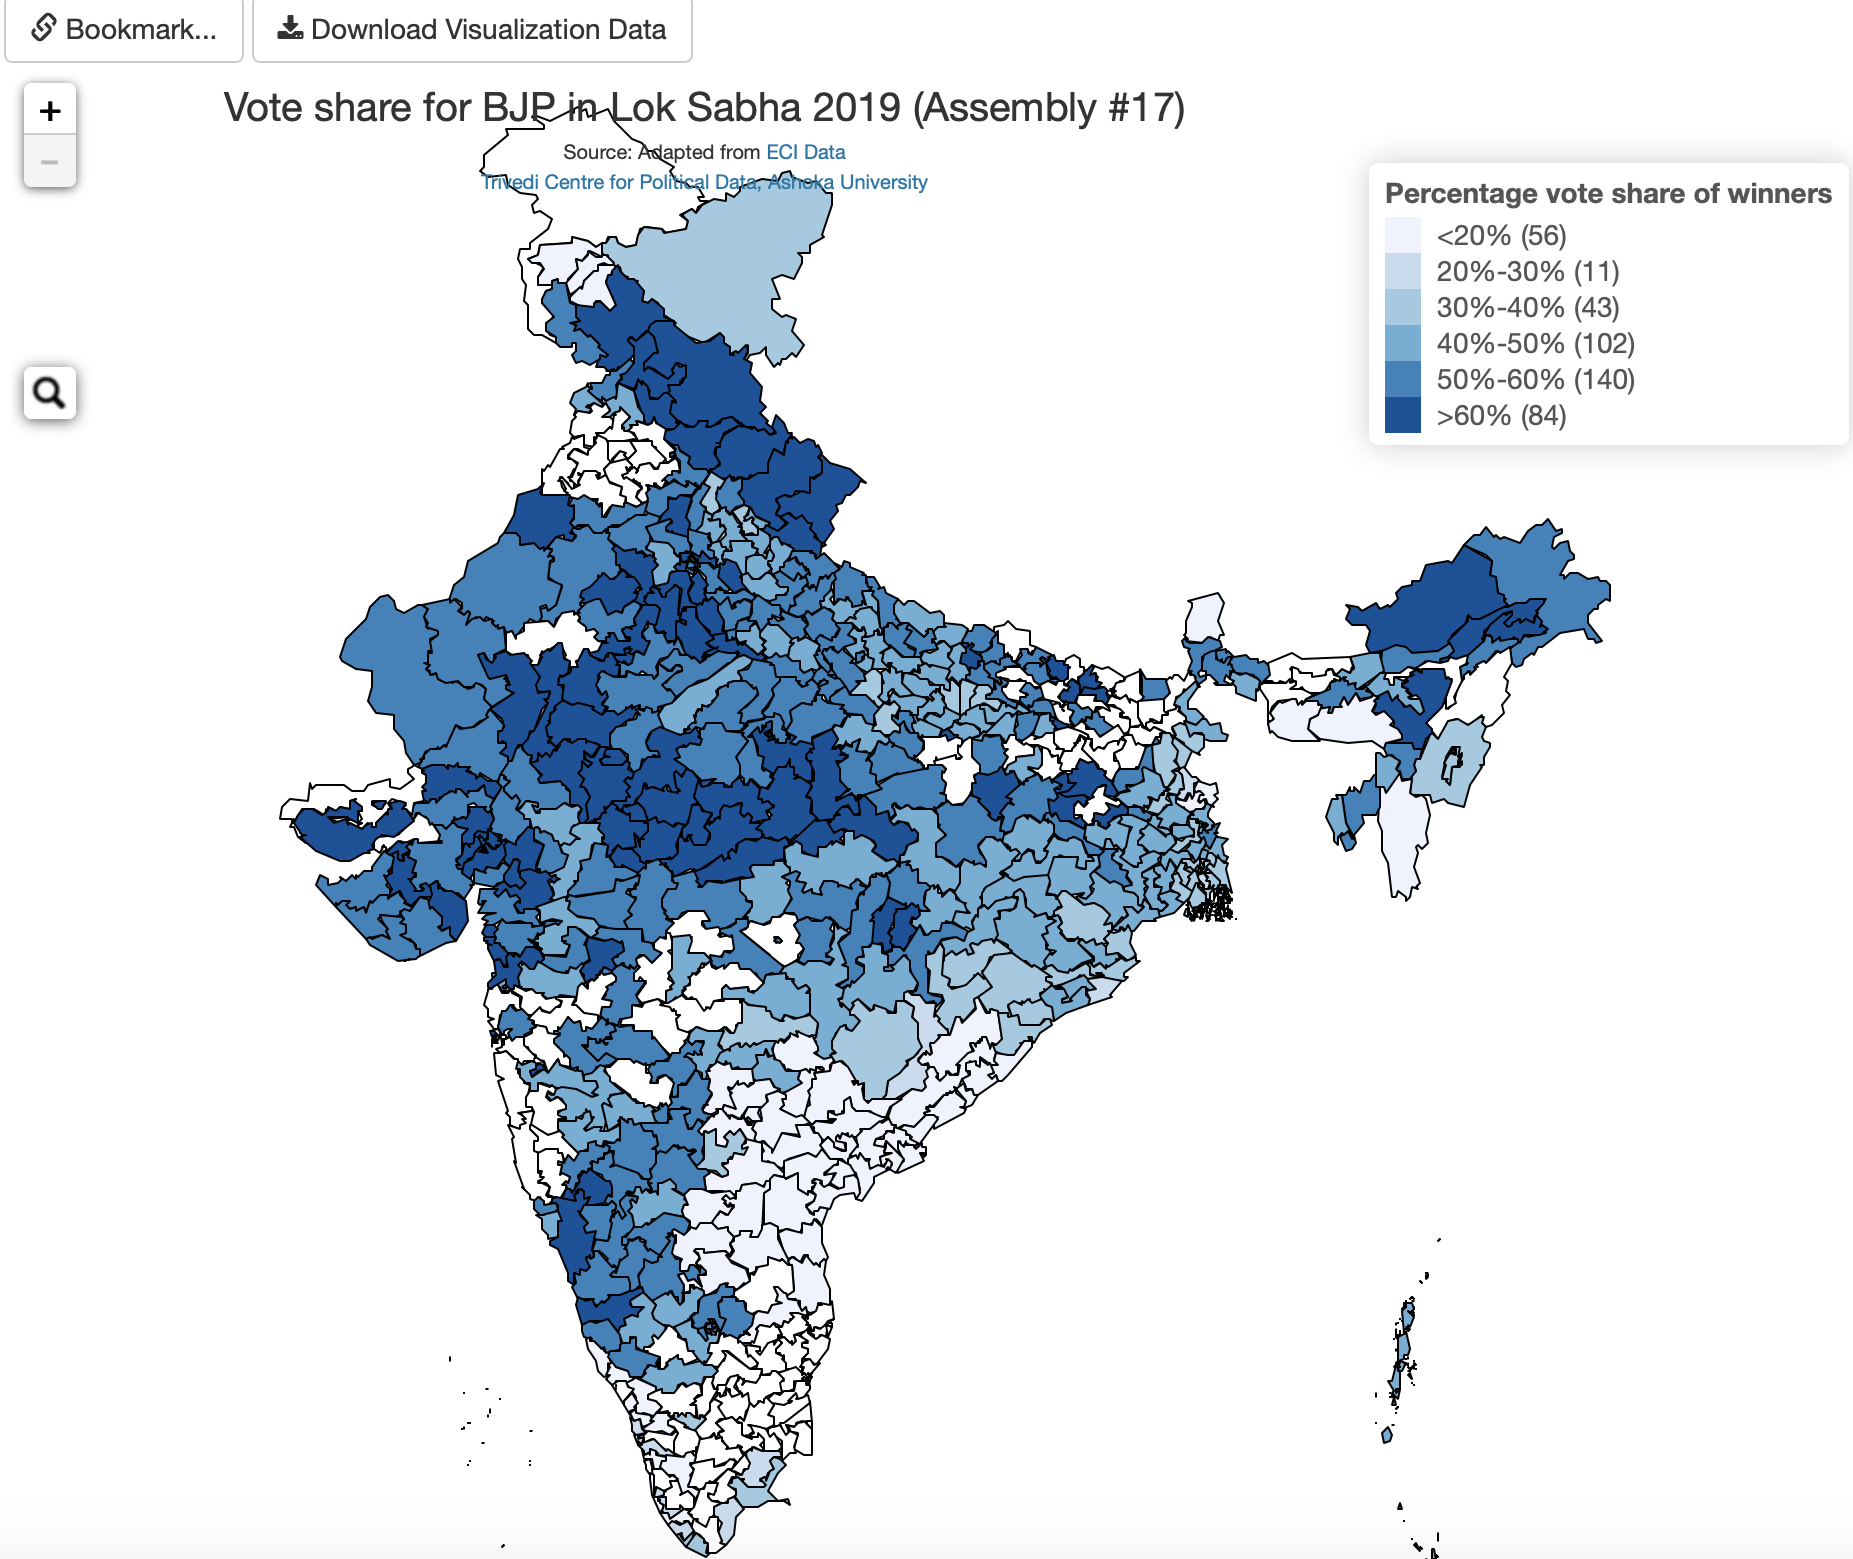
\includegraphics[width=\linewidth]{BJPVoteshare2019}
 \caption{Visualization of constituency-wise vote shares of BJP candidates in the 2019 national elections}
 \label{BJPVS}
 \end{figure}
 
 \begin{figure}
 \centering
 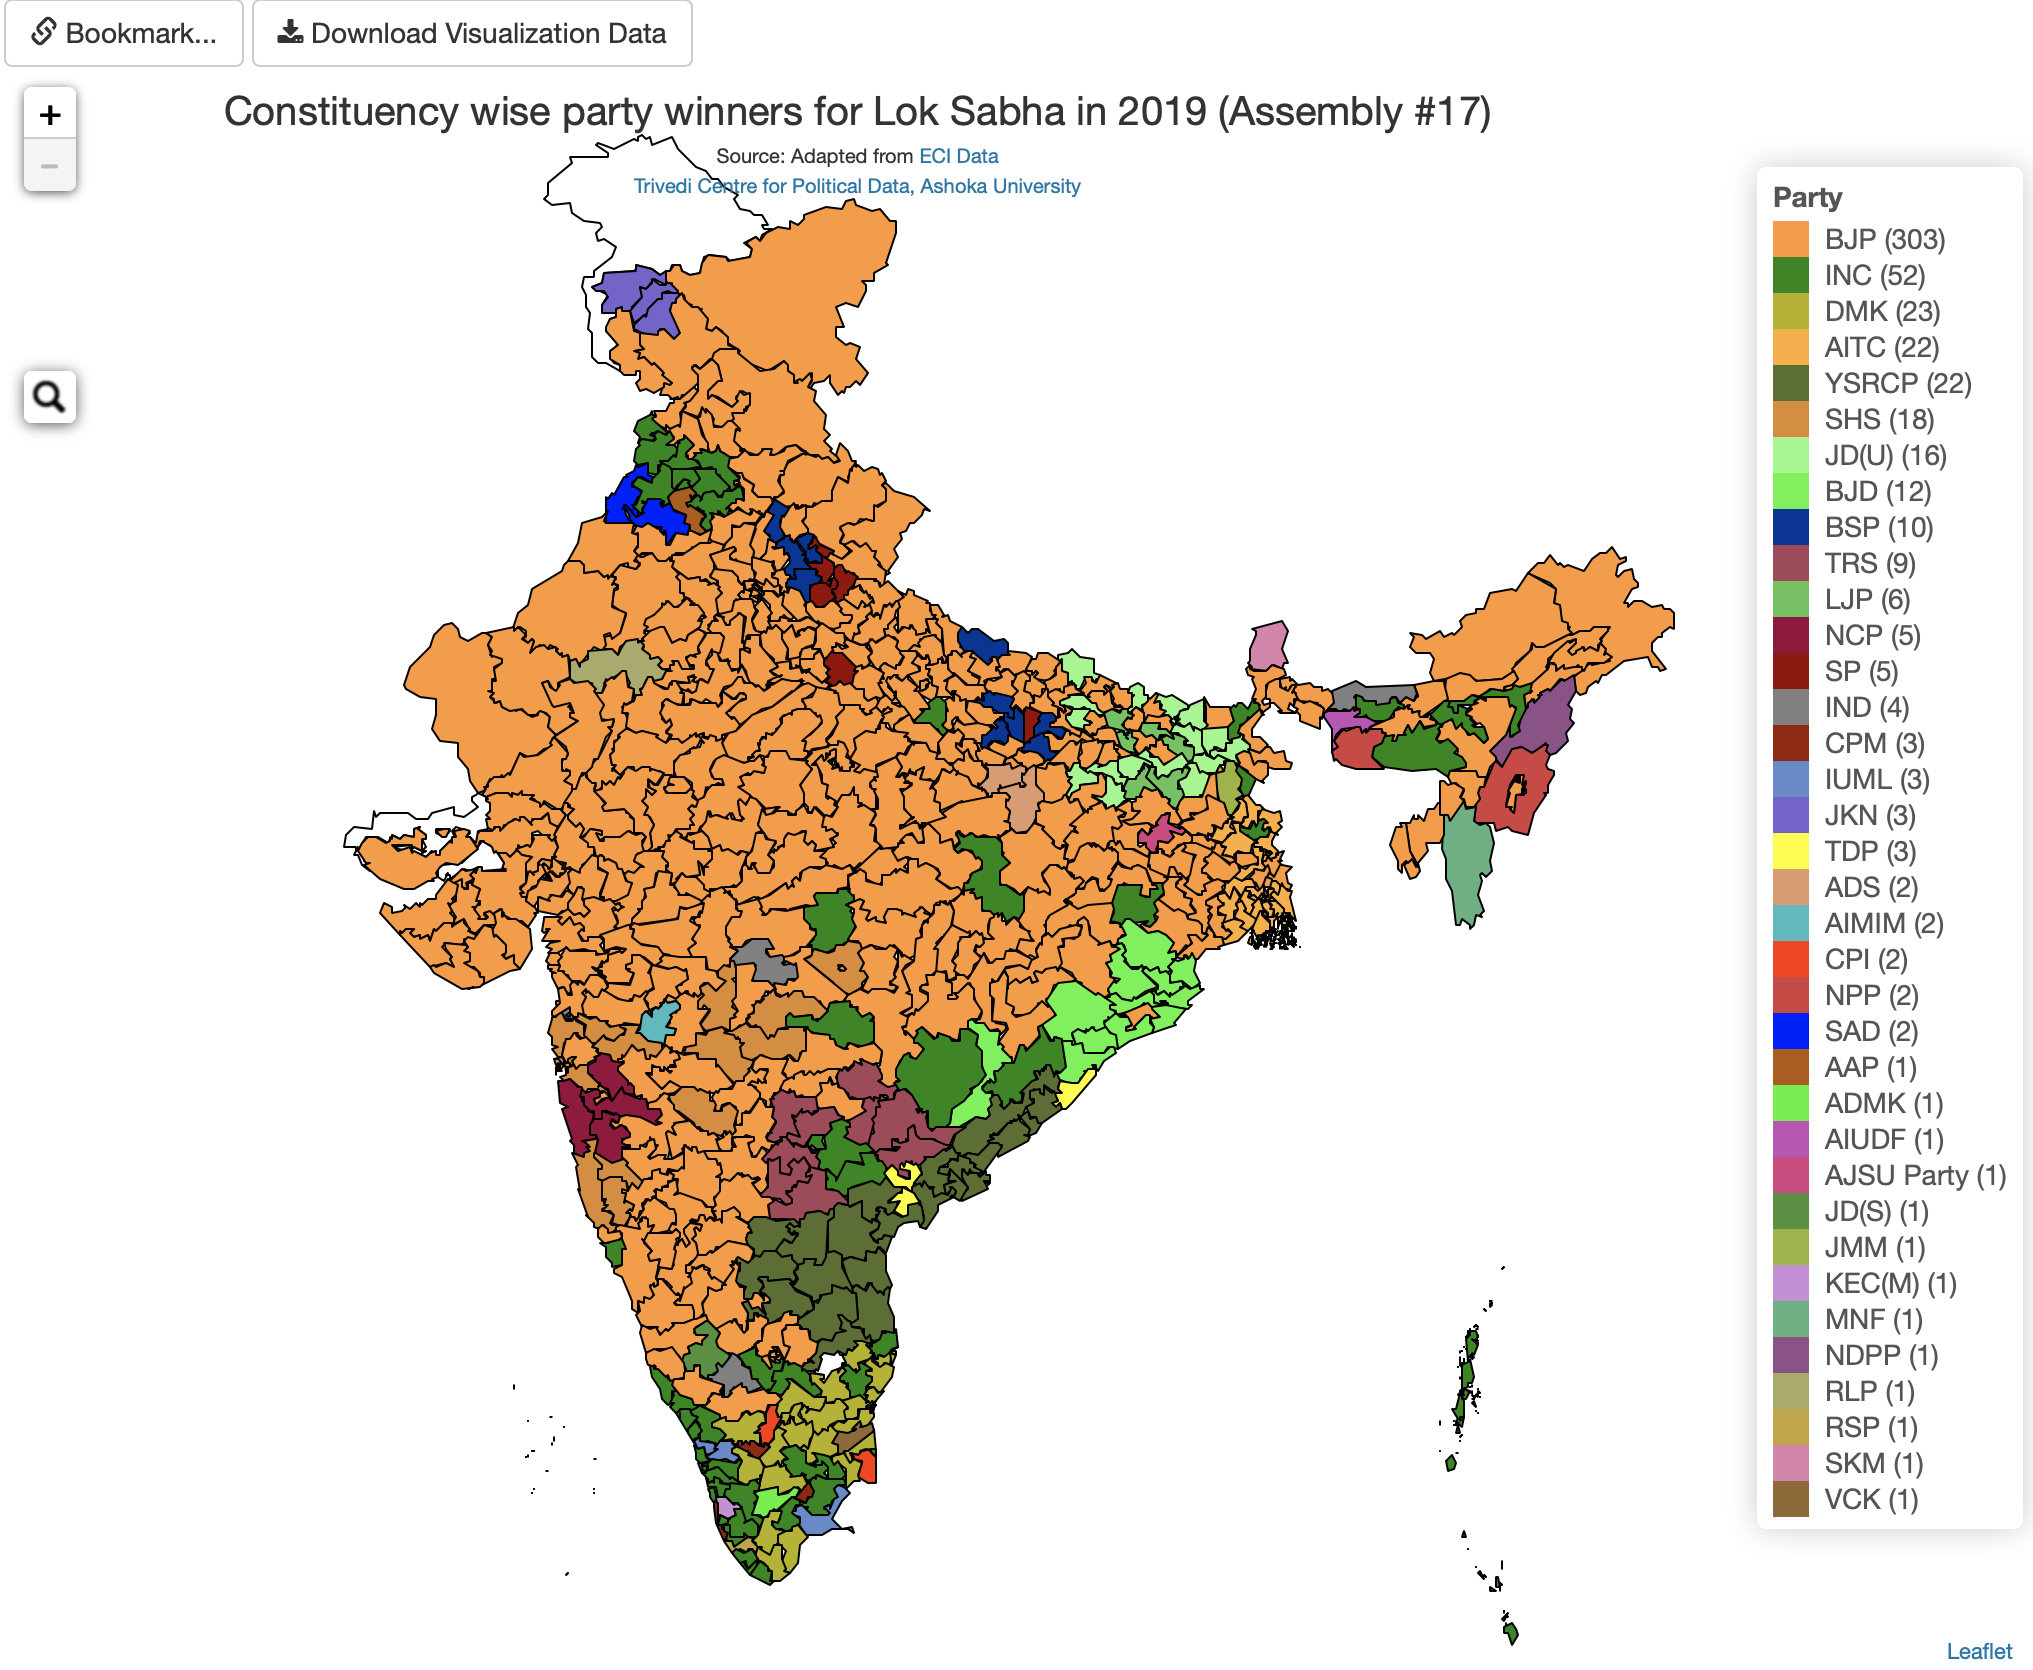
\includegraphics[width=\linewidth]{PartyWinnersMap2019}
 \caption{Visualization of the winning party in the 2019 national elections }
 \label{partyWn}
 \end{figure}
 
 \subsubsection{Incumbency profile}
Indian elections feature candidates who frequently cross over between parties. Candidates' affiliations to parties tend to be based on pragmatic rather than ideological considerations. There is a steady stream of parties splitting and merging, pre-poll and post-poll coalitions, or candidates crossing over from one party to another. There is often an anti-incumbency wave, meaning that a ruling party or legislator may have a disadvantage as voters blame them for poor governance. Assignment of tickets within a party is also an opaque process, with some parties tending to favor loyalists, while others preferring to rotate their candidates. It is therefore very interesting for political scientists to trace the trajectory of individual candidates, and ask who gets nominated, elected, re-nominated, re-elected, etc.

LokDhaba includes a visualization showing career performance of elected members or contestants of a specific assembly. In this visualization, the user can see the complete record of each contestant, such as their current and previous party affiliations and electoral performance. This component is designed to enable the user to view all elected and major-party candidates clustered together by party, while also depicting their party affiliation in the immediately preceding assembly, in order to identify turncoats. Winners and losers are represented by shape, and the shape can be annotated with a single number, either the candidate's number of attempts, or the number of their victories. Upon hovering on a shape, users can view prior contest information and a photograph of the candidate. A search function enables the user to narrow down to a specific person or constituency of interest. Users can also filter down by gender or experience, in order to focus on specific subsets of the candidates.
 
 Fig. \ref{incm_all} shows a snapshot of the winners of the 2019 Parliamentary elections. Fig. \ref{incm_rhl} shows the search for the name "Rahul" and the resulting information on Mr. Rahul Gandhi of the Indian National Congress.
 \begin{figure}
 \centering
 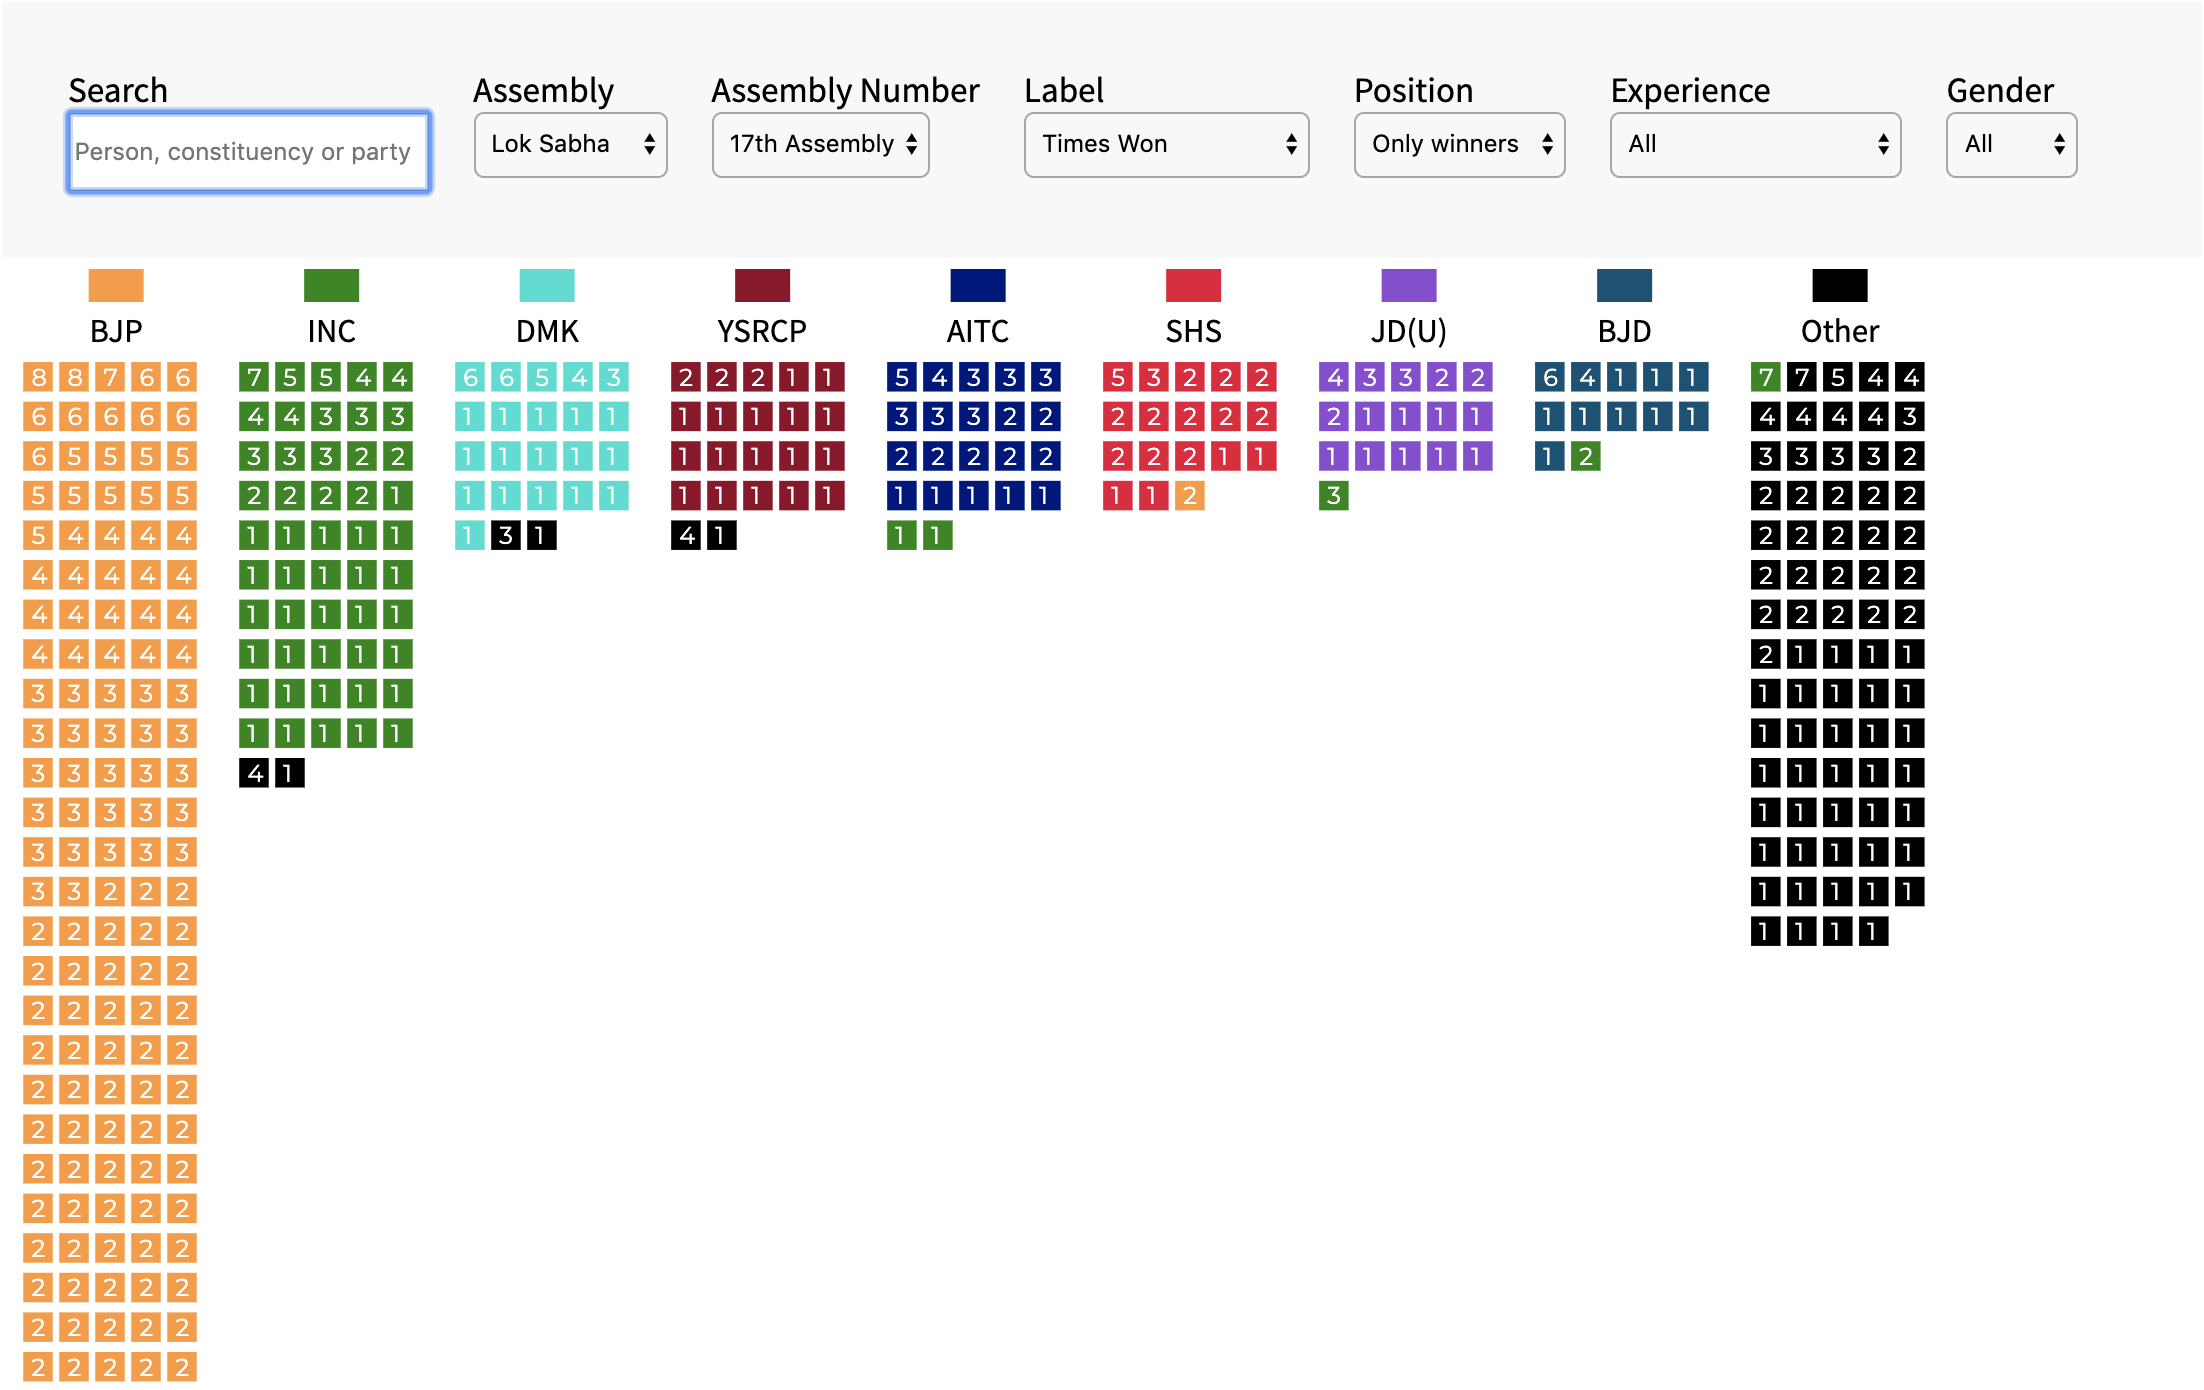
\includegraphics[width=\linewidth]{Incumbency_Profile.png}
 \caption{Incumbency profile of the 2019 national election winners}
 \label{incm_all}
 \end{figure}
 \begin{figure}
 \centering
 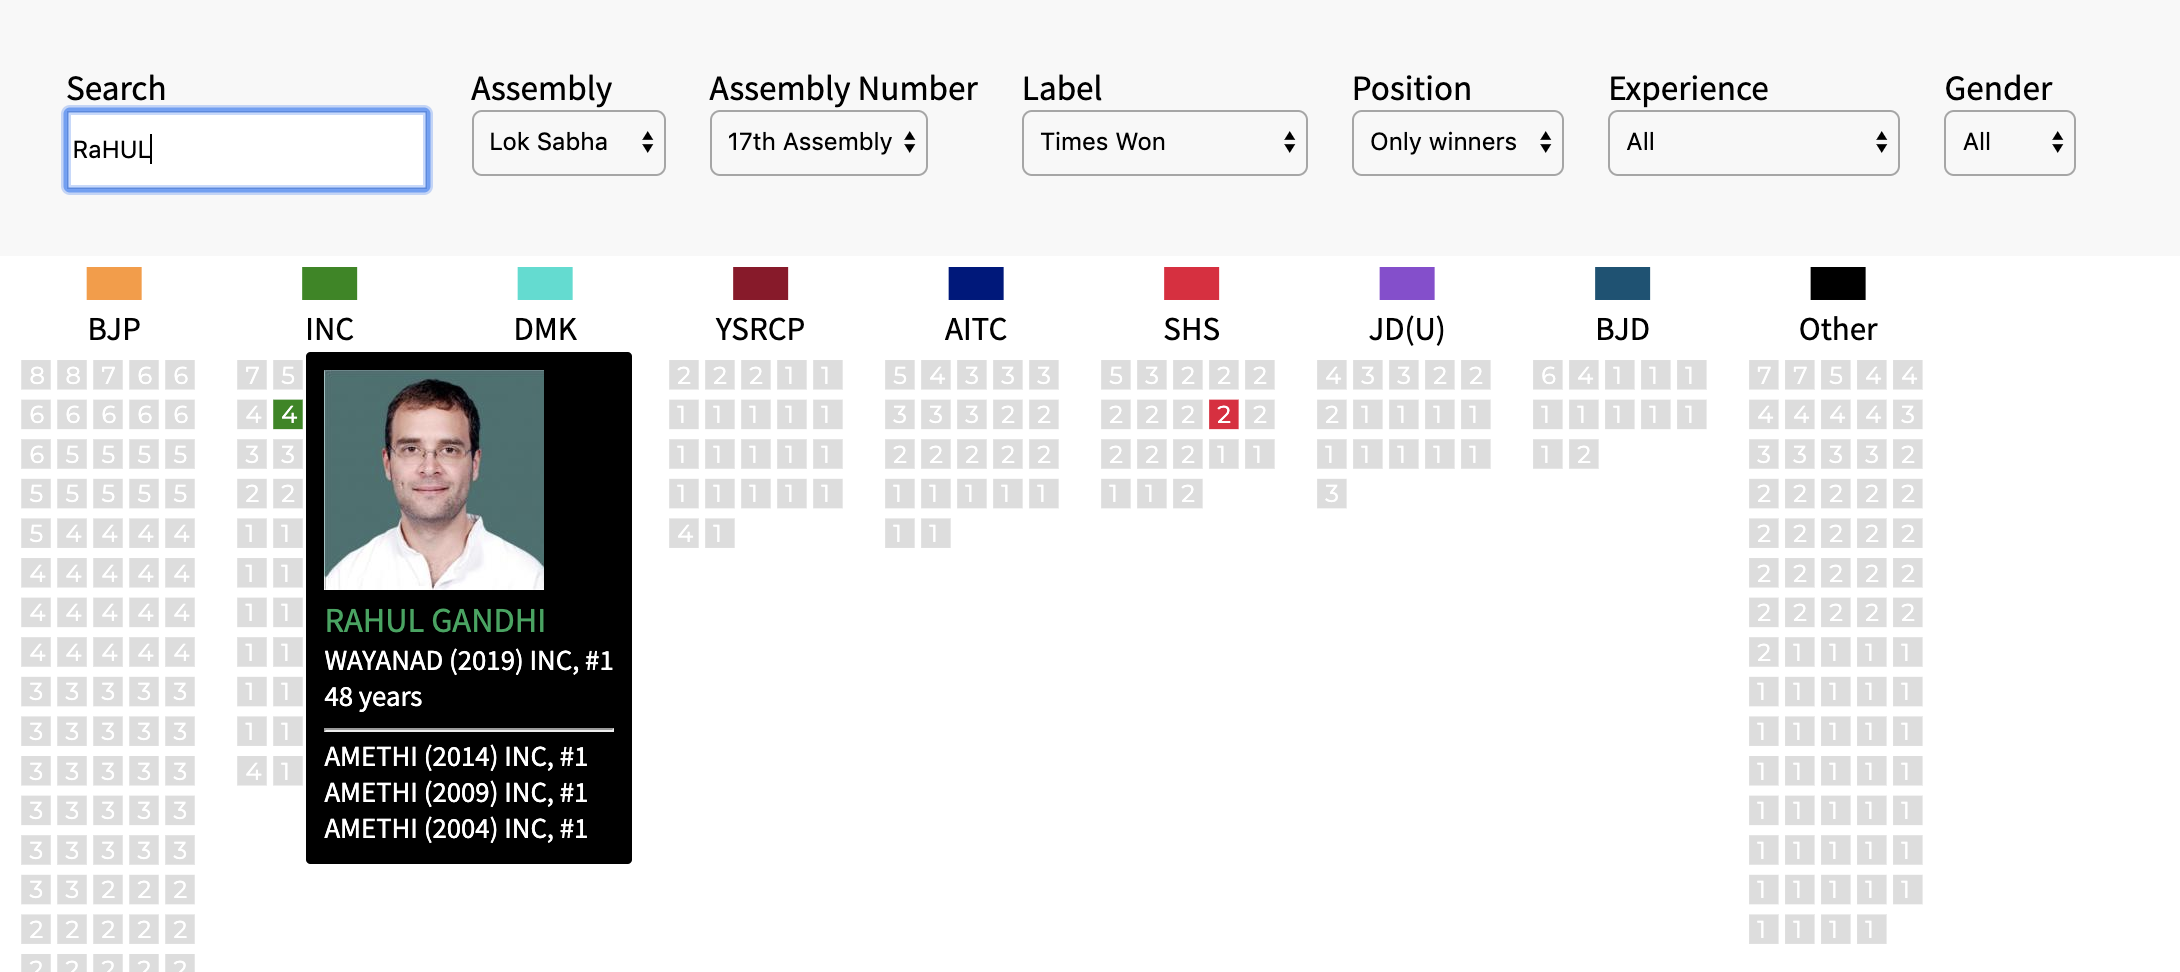
\includegraphics[width=\linewidth]{Incumbency_RG.png}
 \caption{Viewing a candidate's details}
 \label{incm_rhl}
 \end{figure}
 
\section{User Feedback}
To get a sense of the usability of LokDhaba, we conducted a survey with expert political scientists and journalists who have used LokDhaba\footnote{Susmeet Jain and Keshav Joshi led the pilot study.}, and received 13 responses. Most users report using LokDhaba for research purposes (63.6\%). Unsurprisingly, close to half of our respondents use the platform around the time of an election (45.5\%). They report downloading more charts (90\%) than maps (54.5\%). Most users prefer working on LokDhaba on a computer rather than a mobile device (81.8\% and 36.4\% respectively). Most users report that it is easy for them to browse the data (81.9\%). However, only 63.6\% of the users agreed that the visualizations are effective and only 54.5\% report that the incumbency profile is intuitive.

Google Analytics statistics for the period May 2019-2020 (when there was a national election) showed that there were 10,284 unique users, with 15,383 sessions. Most of the traffic comes to LokDhaba directly (73.95\%), followed by organic search (12.42\%), followed by social channels like Twitter or Facebook (10.66\%), and referrals from other media sources (3\%). 89\% of users are from India, 5\% from the United States, and 2\% from the United Kingdom. The rest are from Singapore, Canada, France, U.A.E, Germany and a few other parts of the world.

\section{Conclusions and Impact}

In this paper, we have described the challenges encountered in assembling and maintaining a high-value longitudinal dataset. We have proposed some solutions, including new tools and best practices to meet these challenges that we hope will be useful in other domains as well.

Apart from research contributions, LokDhaba has had substantial impact on the state of the practice. We describe some of these impact areas below.

\subsection{Application}

The first contribution to the practice is that of an open source application with a simple user interface to browse and visualize electoral data. The data as well as the web application is freely available for download. The LokDhaba application code is maintained as a freely accessible open source git repository\cite{lokdhabaRepo} and can easily be used for other electoral datasets with a First Past the Post system.

\subsection{Study of Indian Elections}

LokDhaba makes several key contributions to the study of Indian elections. The first is that it pulls together information from multiple sources with varying formats. Building from ECI's statistical reports, LokDhaba has variables at both the constituency and candidate level. We have also integrated these with data on individuals' assets and crime records. In the future, we expect to bring together several indicators of social and political behavior, with the aim of enabling more research on political candidates.

Secondly, through the assignment of unique identifiers, we are able to track both politicians and political parties over time and space. Researchers can now ask a wider array of questions about the career trajectory of politicians, when they defect, to which party and their subsequent performance. 

Finally, data on bye-elections has been an important but neglected part of the electoral process. Bye-elections can now be empirically studied and evaluated along with the main elections.

\subsection{Training and Outreach}

LokDhaba also enables several initiatives which we broadly classify as outreach. The first is as a source of data for other data dissemination initiatives. We are aware of at least two repositories - Jaano India\footnote{https://jaanoindia.swaniti.org/} and the Constituency-Level Election Archive (CLEA) at the University of Michigan\footnote{http://www.electiondataarchive.org./} - that use the data provided by LokDhaba.

An unexpectedly pleasant use of LokDhaba has been for instruction in the classroom and for training inter-disciplinary students. LokDhaba is used to train and encourage students to think critically about data, spot anomalies, and analyze long-term patterns and trends. It is used during lectures in classes and in an annual summer school attended by undergraduate and post-graduate students, professionals and journalists. Our outreach demonstrates to our partners that building datasets is a non-trivial process and requires careful work in all phases of the data lifecycle.

\section{Future Work}

The LokDhaba dataset is being continually updated and is expanding in terms of integration with other datasets. We plan to build more map-based visualizations, including some that allow longitudinal comparison of results (e.g., vote share of parties across successive elections). We also need to improve our mapping infrastructure and get more authoritative sources of geo-spatial data. We welcome collaboration with groups that need to work with election results data.

%%
%% The acknowledgments section is defined using the "acks" environment
%% (and NOT an unnumbered section). This ensures the proper
%% identification of the section in the article metadata, and the
%% consistent spelling of the heading.
\begin{acks}
We thank the Trivedi Centre for Political Data team: Saloni Bhogale,  Basim-U-Nissa, Kirti, Venkat Prasath, Rajkamal Singh, Sudesh Singh, Shivangi Tikekar, and  Gilles Verniers, as well as Francesca Jensenius, for useful inputs in the design and implementation of LokDhaba.

\end{acks}

%%
%% The next two lines define the bibliography style to be used, and
%% the bibliography file.
\bibliographystyle{ACM-Reference-Format}
\bibliography{sample}

%%
%% If your work has an appendix, this is the place to put it.

\end{document}
\endinput
%%
%% End of file `sample-authordraft.tex'.
